\documentclass[11pt]{article}

\usepackage{amsfonts,amsmath,amssymb,amsthm}
\usepackage[normalem]{ulem} % temporary for strikeout math
\usepackage{enumerate}
\usepackage[shortlabels,inline]{enumitem}
\usepackage{wrapfig}

\usepackage[lined,noend]{algorithm2e}
\usepackage{tabularx}
\usepackage{colortbl}
\usepackage{adjustbox}
\DontPrintSemicolon

\PassOptionsToPackage{hyphens}{url}
\usepackage{fullpage}
\usepackage{hyperref}
\usepackage{xcolor}
\usepackage{xifthen}
\usepackage{placeins}
\usepackage{pifont}
\usepackage{multirow}
\usepackage{tikz}
\usepackage{pgfplots}
\usepackage[framemethod=tikz]{mdframed} % and thus tikz
\usepackage[font=small]{caption}

\usepackage{authblk}

% footnotes in table and tabular
\usepackage{footnote}
\makesavenoteenv{tabular}
\makesavenoteenv{table}
\makesavenoteenv{figure}

\usepackage{stmaryrd} % fancy double square brackets
\usepackage{todonotes}

\setcounter{tocdepth}{2} % Override LLNCS

% ==== Hydra Macros ====

% NOTE: New macro file; please copy and keep organized macros from
% macros_old.tex as needed.  Hopefully, this will result in tidier
% macros file.
%
% Index:
% - Misc
% - General
% - Theorem Environments
% - Multisignatures
% - Transactions
% - State Machines
% - Head Protocol
% - On-Chain Verification
% - Algorithms
% - Merkle-Patricia Trees

% === engineering ===
\newcommand{\undefined}{\mathrm{undef}}


% === Misc ===

\newcommand{\algoskip}{\vspace{4pt}}

\newcommand{\ignore}[1]{}

\newcommand{\TODO}[1]{
  \if\relax\detokenize{#1}\relax
    \textcolor{red}{TODO}
  \else
    \textcolor{red}{ {#1}}
  \fi
}

\newcommand{\fail}{\mbox{fail}}

% from https://www.overleaf.com/latex/examples/simple-stylish-box-design/stzmmcshxdng
\definecolor{main}{HTML}{5989cf}    % setting main color to be used
\definecolor{sub}{HTML}{cde4ff}     % setting sub color to be used
\newtcolorbox{boxM}{
    fontupper = \color{white},
    rounded corners,
    arc = 6pt,
    colback = main!80, 
    colframe = main, 
    boxrule = 0pt, 
    bottomrule = 4.5pt,
    enhanced,
    fuzzy shadow = {0pt}{-3pt}{-0.5pt}{0.5pt}{black!35}
}

% In figures, this makes algorithms work with option [H] despite
% double-column format
% https://tex.stackexchange.com/questions/82271/multiple-algorithm2e-algorithms-in-two-column-documents
\makeatletter
\newcommand{\removelatexerror}{\let\@latex@error\@gobble}
\makeatother

\newcommand{\md}{\textsf{-}}

\newcommand{\fst}[1]{#1^{\text{st}}}
\newcommand{\snd}[1]{#1^{\text{nd}}}
\newcommand{\trd}[1]{#1^{\text{rd}}}
\newcommand{\ith}[1]{#1^{\text{th}}}

\newcommand{\eps}{\varepsilon}
\newcommand{\mc}{\mathcal}

\DeclareMathOperator*{\argmax}{arg\,max}
\DeclareMathOperator*{\argmin}{arg\,min}


% === General ===
\newcommand{\ol}[1]{\overline{#1}}

\newcommand{\true}{\mathtt{true}}
\newcommand{\false}{\mathtt{false}}

\newcommand{\spara}{k}

\newcommand{\nop}{n}
\newcommand{\party}{\mathsf p}
\newcommand{\parties}{\mathcal{P}}

\newcommand{\adv}{\ensuremath{\mathcal{A}}}
\newcommand{\att}{\adv}
\newcommand{\advLive}{\ensuremath{\mathcal{A}}_{\mathsf L}}

\newcommand{\propName}{\textsc}

\newcommand{\hout}[1]{h_{\mathsf{out},#1}}
\newcommand{\hrest}{h_{\mathsf{rest}}}

\newcommand{\es}{\eps}

\newcommand{\hash}{\mathsf{hash}}
\newcommand{\bytes}{\mathsf{bytes}}


% === Theorem Environments ===

\newtheoremstyle{putaneffinperiod}% name of the style to be used
  {\topsep}% measure of space to leave above the theorem. E.g.: 3pt
  {\topsep}% measure of space to leave below the theorem. E.g.: 3pt
  {\itshape}% name of font to use in the body of the theorem
  {0pt}% measure of space to indent
  {\bfseries}% name of head font
  {.}% punctuation between head and body
  {1em}% space after theorem head; " " = normal interword space
  {\thmname{#1}\thmnumber{ #2}\thmnote{ (#3)}}
\theoremstyle{putaneffinperiod}

\newtheorem{theorem}{Theorem}
% \numberwithin{theorem}{chapter}
\newtheorem{lemma}[theorem]{Lemma}
\newtheorem{corollary}[theorem]{Corollary}
\newtheorem{proposition}[theorem]{Proposition}
\newtheorem{claim}[theorem]{Claim}
\newtheorem{definition}{Definition}
% \numberwithin{definition}{chapter}
\newtheorem{invariant}{Invariant}
\newtheorem{axiom}[theorem]{Axiom}
\newtheorem{postulate}{Postulate}
\theoremstyle{definition}
\newtheorem{example}{Example}
\newtheorem{construction}{Construction}


% === Transactions ===

\newcommand{\tyBool}{\mathbb{B}}
\newcommand{\tyNatural}{\mathbb{N}}
\newcommand{\tyInteger}{\mathbb{Z}}
\newcommand{\tyData}{\mathsf{Data}}
\newcommand{\tyBytes}{\mathbb{H}}

\newcommand{\datum}{\delta} % a datum
\newcommand{\redeemer}{\rho} % a redeemer

\newcommand{\txContext}{\gamma} % validation context
\newcommand{\tyContext}{\Gamma} % type of contexts

\newcommand{\val}{\mathsf{val}} % a value
\newcommand{\tyValue}{\mathsf{Val}} % type of values

\newcommand{\tx}{\mathrm{tx}}
\newcommand{\txA}{\mathrm{txA}}
\newcommand{\txB}{\mathrm{txB}}
\newcommand{\validTx}{\mathsf{valid\md{}tx}}
\newcommand{\applytx}{\circ}
\newcommand{\Reach}{\mathsf{Reach}}

\newcommand{\txTx}{\mathit{tx}}			% transaction value
\newcommand{\txTxTy}{\mathit{Tx}}		% transaction type
\newcommand{\txCIdTy}{\mathit{CId}}		% currency identifier type
\newcommand{\txTokenTy}{\mathit{Token}}	        % currency token type
\newcommand{\txKeys}{\kappa} % (public) keys signing the tx
\newcommand{\tyKeys}{\mathcal{K}^*} % type of keys
\newcommand{\txOutRef}{\mathsf{out\md{}ref}}
\newcommand{\txInputs}{\mathcal{I}} % set of inputs
\newcommand{\tyInputs}{\mathcal{I}^*} % type of input sets
\newcommand{\txOutputs}{\mathcal{O}} % list of outputs
\newcommand{\tyOutputs}{\mathcal{O}^{\underline{*}}} % type of output lists
\newcommand{\txMint}{\mathsf{mint}} % minted value
\newcommand{\txID}{\mathit{txID}}
\newcommand{\ID}{\mathsf{ID}}
\newcommand{\txIdx}{\mathit{txIdx}}
\newcommand{\txR}{r}
\newcommand{\txRmin}{r_{\mathsf{min}}}
\newcommand{\txRmax}{r_{\mathsf{max}}}

\newcommand{\txIpend}{i_{\mathsf{pend}}}
\newcommand{\txIpendSet}{I_{\mathsf{pend}}}

\newcommand{\Tset}{T}
\newcommand{\Uset}{U}
\newcommand{\Uinit}{\Uset_{0}}
\newcommand{\Ufinal}{\Uset_{\mathsf{final}}}

\newcommand{\recordUTxO}{\mathsf{recordUTxO}}

% === Multisignatures ===

\newcommand{\ms}{\mathsf{MS}}

\newcommand{\msSetup}{\mathsf{MS\md{}Setup}}
\newcommand{\msKeyGen}{\mathsf{MS\md{}KG}}
\newcommand{\msSign}{\mathsf{MS\md{}Sign}}
\newcommand{\msVfy}{\mathsf{MS\md{}Verify}}
\newcommand{\msComb}{\mathsf{MS\md{}ASig}}
\newcommand{\msCombVK}{\mathsf{MS\md{}AVK}}
\newcommand{\msCombVfy}{\mathsf{MS\md{}AVerify}}

\newcommand{\msParams}{\Pi}
\newcommand{\msSig}{\sigma}
\newcommand{\msSigL}{\Sigma}
\newcommand{\msCSig}{\tilde\sigma}
\newcommand{\msVK}{k^{ver}}
\newcommand{\msCVK}{\tilde{k}}
\newcommand{\msVKL}{\mathcal{V}}
\newcommand{\msSK}{k^{sig}}
\newcommand{\msMsg}{m}

\newcommand{\initial}[1]{\dot{#1}}
%\newcommand{\chain}[1]{\dot{#1}}
\newcommand{\sVK}{k_{\pu}}
\newcommand{\sVKI}[1]{k_{#1,\pu}}
\newcommand{\sVKII}[1]{\initial{k}_{#1,\pu}}
\newcommand{\sSK}{k_{\pr}}
\newcommand{\sSKI}[1]{k_{#1,\pr}}
\newcommand{\sSKII}[1]{\initial{k}_{#1,\pr}}

% === State Machines ===

\newcommand{\cemS}{S_{\textsc{cem}}}
\newcommand{\cemI}{I_{\textsc{cem}}}
\newcommand{\cemIn}{i_{\textsc{cem}}}
\newcommand{\cemOut}{o_{\textsc{cem}}}
\newcommand{\cemValidator}{\nu_{\textsc{cem}}}
\newcommand{\cemDatum}{\datum_{\textsc{cem}}}
\newcommand{\cemRedeemer}{\redeemer_{\textsc{cem}}}
\newcommand{\cemFinal}{\mathit{final}_{\textsc{cem}}}
\newcommand{\cemStep}{\mathit{step}_{\textsc{cem}}}
\newcommand{\cemStepRel}[4]{{#1}\overset{#2}\longrightarrow(#3, #4)}
\newcommand{\cemTxCon}{\tx^\equiv}

\newcommand{\cid}{\mathsf{cid}} % head id / currency id

\newcommand{\st}{\mathsf{ST}}
\newcommand{\pt}{\mathsf{PT}}

% == Transactions ==

\newcommand{\mtxInit}{\textit{init}}
\newcommand{\mtxCom}{\textit{commit}}
\newcommand{\mtxCommit}{\textit{commit}}
\newcommand{\mtxCCom}{\textit{collectCom}}
\newcommand{\mtxCollect}{\textit{collectCom}}
\newcommand{\mtxIncrement}{\textit{increment}}
\newcommand{\mtxDecrement}{\textit{decrement}}
\newcommand{\mtxAbort}{\textit{abort}}
\newcommand{\mtxClose}{\textit{close}}
\newcommand{\mtxContest}{\textit{contest}}
\newcommand{\mtxFinalize}{\textit{finalize}}
\newcommand{\mtxFanout}{\textit{fanout}}
\newcommand{\mtxSplit}{\textit{split}}
\newcommand{\mtxCSN}{\textit{collectSN}}
\newcommand{\mtxCHT}{\textit{collectHT}}
\newcommand{\mtxSN}{\textit{SN}}
\newcommand{\mtxHT}{\textit{HT}}

% == States ==

\newcommand{\stInitial}{\mathsf{initial}}
\newcommand{\stOpen}{\mathsf{open}}
\newcommand{\stClosed}{\mathsf{closed}}
\newcommand{\stSnap}{\mathsf{newestSN}}
\newcommand{\stFinal}{\mathsf{final}}

\newcommand{\hMT}{h_{\mathsf{MT}}}
\newcommand{\piMT}{\pi_{\mathsf{MT}}}
\newcommand{\cPer}{T}
\newcommand{\Tfinal}{T_{\mathsf{final}}}
\newcommand{\Tsnapshot}{T_{\mathsf{newestSN}}}
\newcommand{\contesters}{\mathcal C}


% == Inputs ==

\newcommand{\stCollect}{\mathsf{collect}}
\newcommand{\stClose}{\mathsf{close}}
\newcommand{\stContest}{\mathsf{contest}}
\newcommand{\stFanout}{\mathsf{fanout}}
\newcommand{\stAbort}{\mathsf{abort}}


% == Validators ==

\newcommand{\muHead}{\mu_\mathsf{head}}
\newcommand{\nuHead}{\nu_\mathsf{head}}
\newcommand{\nuInitial}{\nu_\mathsf{initial}}
\newcommand{\nuCommit}{\nu_\mathsf{commit}}
\newcommand{\nuSnap}{\nu_\mathsf{SN}}
\newcommand{\nuNewname}{\nu_\mathsf{newestSN}}
\newcommand{\nuHang}{\nu_\mathsf{HT}}
\newcommand{\nuFinal}{\nu_\mathsf{final}}


% === Head Protocol ===

% == Algorithms ==

\newcommand{\HP}{\mathsf{HP}}
\newcommand{\hpSetup}{\mathsf{Setup}}
\newcommand{\hpKG}{\mathsf{KeyGen}}
\newcommand{\hpAgg}{\mathsf{Agg}}
\newcommand{\hpProt}{\mathsf{Prot}}


% == Protocol ==

\newcommand{\hpInit}{\mathtt{init}}
\newcommand{\hpNew}{\mathtt{new}}
\newcommand{\hpSeen}{\mathtt{seen}}
\newcommand{\hpConf}{\mathtt{conf}}
\newcommand{\hpClose}{\mathtt{close}}
\newcommand{\hpCont}{\mathtt{cont}}
\newcommand{\hpFO}{\mathtt{fanOut}}

\ignore{
\newcommand{\obj}{\Omega}

\newcommand{\certreq}{\ensuremath{\mathtt{sigReq}}}
\newcommand{\certack}{\ensuremath{\mathtt{sigAck}}}
\newcommand{\certconf}{\ensuremath{\mathtt{sigConf}}}

\newcommand{\abortreq}{\ensuremath{\mathsf{abortReq}}}

\newcommand{\init}{\mathbf{Init}}
\newcommand{\gencert}{\mathbf{GenCert}}

\newcommand{\txobj}{\mathsf{txo}}
\newcommand{\genobj}{\mathsf{obj}}
\newcommand{\genset}{\mathsf{ObjSet}}
\newcommand{\gentxobj}{\mathsf{GenTxObj}}
\newcommand{\stateobj}{\ensuremath{u}}
\newcommand{\ack}{\mathsf{ack}}
}

% == Variables ==
\newcommand{\pu}{\mathsf{ver}}
\newcommand{\pr}{\mathsf{sig}}


\newcommand{\hpParams}{\Sigma}
\newcommand{\hpPu}{K_{\pu}}
\newcommand{\hpPuv}{\underline{K}_\pu}
\newcommand{\hpPui}[1]{K_{\pu,#1}}
\newcommand{\hpPr}{K_{\pr}}
\newcommand{\hpPri}[1]{K_{\pr,#1}}

\newcommand{\hpAK}{\tilde{k}_{\mathsf{H}}} % Aggregated hydra key
\newcommand{\hppuv}{\underline{k}_C} % List of cardano keys
\newcommand{\keyHash}{k^{\#}} % Some verification key hash

\newcommand{\hpPuvInit}{\initial{\underline{K}}_\pu}

\newcommand{\hpAKchain}{\hpAK^{\mathsf{chain}}}
\newcommand{\hpAKinit}{\hpAK^{\mathsf{setup}}}

%\newcommand{\initial}{\mathsf{init}}
\newcommand{\daPuII}[1]{\initial{K}_{#1,\pu}}
\newcommand{\daPrII}[1]{\initial{K}_{#1,\pr}}
%\newcommand{\sVKI}{\mathsf{vk}^{\initial}}
%\newcommand{\sSKI}{\mathsf{sk}^{\initial}}

\newcommand{\hppuvinit}{\initial{\underline{k}}_\pu}


\newcommand{\hats}{\hat s}
\newcommand{\bars}{\overline s}
\newcommand{\hatmU}{\hat {\mathcal U}}
\newcommand{\barmU}{\overline {\mathcal U}}
\newcommand{\mL}{{\mathcal L}}
\newcommand{\hatmL}{\hat {\mathcal L}}
\newcommand{\barmL}{\overline {\mathcal L}}
\newcommand{\mT}{{\mathcal T}}
\newcommand{\hatmT}{\hat {\mathcal T}}
\newcommand{\barmT}{\overline {\mathcal T}}
\newcommand{\hatmDT}{\Delta\hat {\mathcal T}}
\newcommand{\hatmR}{\hat {\mathcal R}}
\newcommand{\mH}{{\mathcal H}}

\newcommand{\TR}{T_{\mathsf R}}
\newcommand{\tTR}{\tilde T_{\mathsf R}}
\newcommand{\tR}{\tilde R}

\newcommand{\hpSigs}{S}

\newcommand{\txo}{\mathsf{tx}}


% == Commands ==

\newcommand{\hpRG}{\mathtt{req}}
\newcommand{\hpAG}{\mathtt{ack}}
\newcommand{\hpCG}{\mathtt{conf}}

\newcommand{\hpRT}{\mathtt{reqTx}}
\newcommand{\hpAT}{\mathtt{ackTx}}
\newcommand{\hpCT}{\mathtt{confTx}}

\newcommand{\hpNS}{\mathtt{newSn}}
\newcommand{\hpRS}{\mathtt{reqSn}}
\newcommand{\hpAS}{\mathtt{ackSn}}
\newcommand{\hpCS}{\mathtt{confSn}}


% == Functions ==

\newcommand{\Txo}{\mathsf{txObj}}
\newcommand{\Sno}{\mathsf{snObj}}
\newcommand{\ApplyMax}{\mathsf{uApplyMax}}

\newcommand{\hpLdr}{\mathsf{leader}}
\newcommand{\hpMT}{\mathsf{maxTxos}}

\newcommand{\conf}{\mathsf{conflict}}
\newcommand{\confTx}{\mathsf{conflict\md{}tx}}

% serialisation
\newcommand{\bits}{\mathsf{bits}}

% == Projectors ==

\newcommand{\hpProj}{_{\downarrow (\tx,\msCSig)}}
\newcommand{\hpProjT}{_{\downarrow (\tx)}}
\newcommand{\hpProjH}{_{\downarrow (\hash)}}
\newcommand{\hpProjSig}{_{\downarrow (\msCSig)}}
\newcommand{\hpProjHs}{_{\downarrow (\hash,\msCSig)}}
\newcommand{\hpProjSo}{_{\downarrow (s,\outputset)}}
\newcommand{\hpProjSos}{_{\downarrow (s,\outputset,\msCSig)}}

\renewcommand{\hpProj}{^{\downarrow (\tx,\msCSig)}}
\renewcommand{\hpProjT}{^{\downarrow (\tx)}}
\renewcommand{\hpProjH}{^{\downarrow (\hash)}}
\renewcommand{\hpProjSig}{^{\downarrow (\msCSig)}}
\renewcommand{\hpProjHs}{^{\downarrow (\hash,\msCSig)}}
\renewcommand{\hpProjSo}{^{\downarrow (s,\outputset)}}
\renewcommand{\hpProjSos}{^{\downarrow (s,\outputset,\msCSig)}}


% == Security ==

\newcommand{\Ttilde}{\tilde{T}}
\newcommand{\That}{\hat{T}}
\newcommand{\Tbar}{\overline{T}}
\renewcommand{\Ttilde}{\tilde{S}}
\renewcommand{\That}{\hat{S}}
\renewcommand{\Tbar}{\overline{C}}

\newcommand{\TxNewAll}{{\cal N}}

\newcommand{\Hcont}{H_{\mathsf{cont}}}
\newcommand{\honest}{\mathcal H}
\newcommand{\contSet}{\mathcal C}
\newcommand{\Cchain}{C_{\mathsf{chain}}}
\newcommand{\USN}[1]{\mathrm{SN}_{#1}}
\newcommand{\setSN}[1]{\tilde T_{#1}}
\newcommand{\curSN}[1]{\mathrm{SN}_{\mathsf{cur},#1}}

\newcommand{\INV}[1]{\mathsf{INV}_{#1}}

\newcommand{\atti}[1]{^{(#1)}}

% === Mediator Protocol ===
\newcommand{\gcClientNewHead}{\mathtt{clientNewHead}}
\newcommand{\gcClientTx}{\mathtt{clientTx}}
\newcommand{\gcClientClose}{\mathtt{closeTx}}
\newcommand{\gcChainInitial}{\mathtt{initialTx}}
\newcommand{\gcChainCollectCom}{\mathtt{collectComTx}}
\newcommand{\gcChainClose}{\mathtt{closeTx}}
\newcommand{\gcChainContest}{\mathtt{contestTx}}
\newcommand{\gcChainFanout}{\mathtt{fanoutTx}}
\newcommand{\gcChainAbort}{\mathtt{abortTx}}
\newcommand{\gcChainCommit}{\mathtt{commitTx}}
\newcommand{\gcChainInitialTO}{\mathtt{chainInitialTimeOut}}
\newcommand{\gcChainClosedTO}{\mathtt{chainClosedTimeOut}}

\newcommand{\gcChainRef}{\mathsf{chain}}
\newcommand{\gcClientRef}{\mathsf{client}}
\newcommand{\gcHeadRef}{\mathsf{head}}
\newcommand{\gcChainPost}{\mathsf{postTx}}
\newcommand{\gcUTXOset}{\mathsf{UTxOs}}
\SetKw{Call}{call}


% === On-Chain Verification ===

% == Algorithms and Oracles ==

\newcommand{\ocvInitial}{\mathsf{Initial}}
\newcommand{\ocvFinalize}{\mathsf{Finalize}}
\newcommand{\ocvClose}{\mathsf{Close}}
\newcommand{\ocvContest}{\mathsf{Contest}}
\newcommand{\ocvFinal}{\mathsf{Final}}

\newcommand{\ocvIncrement}{\mathsf{Increment}}
\newcommand{\ocvDecrement}{\mathsf{Decrement}}

\newcommand{\ocvSnapshot}{\mathsf{Snapshot}}
\newcommand{\ocvValidSnap}{\mathsf{ValidSN}}
\newcommand{\ocvValidHang}{\mathsf{ValidHT}}

\newcommand{\ocvClaim}{\mathsf{Claim}}
\newcommand{\ocvAllocate}{\mathsf{Allocate}}
\newcommand{\ocvFanout}{\mathsf{Fanout}}

\SetKwFor{OocvInitial}{$\ocvInitial$}{}{enddo}
\SetKwFor{OocvFinalize}{$\ocvFinalize$}{}{enddo}
\SetKwFor{OocvClose}{$\ocvClose$}{}{enddo}
\SetKwFor{OocvContest}{$\ocvContest$}{}{enddo}
\SetKwFor{OocvFinal}{$\ocvFinal$}{}{enddo}

\SetKwFor{OocvClaim}{$\ocvClaim$}{}{enddo}
\SetKwFor{OocvAllocate}{$\ocvAllocate$}{}{enddo}
\SetKwFor{OocvFanout}{$\ocvFanout$}{}{enddo}


% == Variables ==

\newcommand{\hInit}{\hash_{\mathsf{init}}}
\newcommand{\imax}{i_{\mathsf{max}}}
\newcommand{\symFinal}{\mathtt{final}}


% == Functions ==

\newcommand{\applicable}{\mathsf{applicable}}


% === Algorithms ===

% == Misc ==

% \setlength{\algomargin}{0em}


% == Boxes ==

\newenvironment{algobox}[1]%
{
  \begin{tabularx}{\textwidth}{X c X}
    \hline
    \rowcolor{gray!20} 
    & \textbf{#1} & \\
    \hline
  \end{tabularx}
  
  \vspace{-1.5em}

  \begin{center}
}
{
  \end{center}

  \vspace{-1.5em}

  \begin{tabularx}{\textwidth}{X c X}
    \hline
  \end{tabularx}

  \vspace{0.5em}
}

\newenvironment{walgo}[1]%
{
  \begin{minipage}{#1\linewidth}
    \begingroup
    \removelatexerror% Nullify \@latex@error
    \begin{algorithm}[H]  
}
{
    \end{algorithm}
    \endgroup
  \end{minipage}
}


% == Keywords ==

\SetKwFor{Check}{check}{}{enddo}


% == DA Game ==

%\newcommand{\algoskip}{\vspace{2pt}}

\SetKwIF{If}{ElseIf}{Else}{if}{}{else if}{else}{end if}
\SetKwFor{For}{for}{}{end for}

\SetKwFor{On}{on}{}{enddo}
\SetKwFor{Function}{function}{}{enddo}
\SetKwFor{PFunction}{public function}{}{enddo}
\SetKw{Out}{output}
\SetKw{Req}{require}
\SetKwFor{ForA}{for all}{}{enddo}
\SetKwFor{Wait}{wait}{}{enddo}
\SetKw{KwWait}{wait} % without body
\SetKw{IfI}{if}
\SetKw{ThenI}{then}
\SetKw{ElsI}{else}
\SetKw{FiI}{fi}

\newcommand{\daPID}{\mathsf{ID}}

\newcommand{\daGlobal}{\Sigma}
\newcommand{\daPu}{K_{\pu}}
\newcommand{\daPuV}{\overline K_{\pu}}
\newcommand{\daPuI}[1]{K_{#1,\pu}}
\newcommand{\daPr}{K_{\pr}}
\newcommand{\daPrI}[1]{K_{#1,\pr}}

\newcommand{\daCInit}{\mathtt{init}}
\newcommand{\daCNew}{\mathtt{new}}
\newcommand{\daCSeen}{\mathtt{seen}}
\newcommand{\daCConf}{\mathtt{conf}}
\newcommand{\daCCert}{\mathtt{cert}}
\newcommand{\daCComp}{\mathtt{comp}}

\SetKw{New}{new}
\SetKw{KwOn}{on}
\SetKw{Send}{send}
\SetKw{Multi}{multicast}
\SetKw{PostTx}{postTx}
\newcommand{\Store}{\mathsf{store}}
\newcommand{\Sign}{\mathsf{sign}}
\newcommand{\Combine}{\mathsf{sigCombine}}
\newcommand{\Verify}{\mathsf{SigVerify}}
\newcommand{\Complete}{\mathsf{Complete}}

\newcommand{\hyPu}{\msCVK}
\newcommand{\hyPr}{\msSK}


% === Merkle-Patricia Trees ===

% == Misc ==

\newcommand{\MPTalph}{A}

% == Algorithms ==

\newcommand{\MPTInit}{\mathsf{MPT\md{}Init}}
\newcommand{\MPTHash}{\mathsf{MPT\md{}Hash}}
\newcommand{\MPTMemb}{\mathsf{MPT\md{}Memb}}

\newcommand{\MPTBuild}{\mathsf{MPT\md{}Build}}
\newcommand{\MPTPath}{\mathsf{MPT\md{}Path}}


% == Hash Computations ==

\newcommand{\MPTverMemb}{\mathsf{MPT\md{}VfyMemb}}
\newcommand{\MPTcompRA}{\mathsf{MPT\md{}CompRA}}
\newcommand{\MPTcompSpl}{\mathsf{MPT\md{}CompSpl}}


% == Helpers ==

\newcommand{\CP}{\mathsf{CP}}
\newcommand{\RP}{\mathsf{RP}}
\newcommand{\Proj}{\mathsf{Proj}}
\newcommand{\Sum}{\mathsf{Sum}}
\newcommand{\Size}{\mathsf{Size}}
\newcommand{\First}{\mathsf{First}}


% == Oracles ==

\SetKwFor{MPTAInit}{\sf MPT-Init}{}{enddo}

\SetKwBlock{MPTAHash}{\sf MPT-Hash}{enddo}
\SetKwFor{MPTAMemb}{\sf MPT-Memb}{}{enddo}

\SetKwFor{MPTABuild}{\sf MPT-Build}{}{enddo}
\SetKwFor{MPTAPath}{\sf MPT-Path}{}{enddo}


% == Variables ==

\newcommand{\MPTroot}{h_{\mathsf{root}}}
\newcommand{\MPTnodes}{N}
\newcommand{\MPTpre}{\mathsf{pre}}
\newcommand{\MPTnode}{\mathsf{node}}
\newcommand{\MPTleaf}{\mathsf{leaf}}
\newcommand{\MPTkey}{k}
\newcommand{\MPTvalue}{v}
\newcommand{\MPTaux}{\mathsf{aux}}
\newcommand{\MPTsplit}{\mathsf{split}}




% == MF ==
\newcommand{\mf}[1]{{\color{red} {#1}}}
% \newcommand{\mfold}[1]{{\color{red}\sout{#1}}}
% \newcommand{\mfreplace}[2]{{\color{red}\sout{#1} {#2}}}
\newcommand{\symdif}{\stackrel{\cdot}{\cup}}
\newcommand{\defeq}{\stackrel{\triangle}{=}}
\newcommand{\sigmaterial}{\Phi}

\newcommand{\dparagraph}[1]{\smallskip\noindent\textbf{#1}}

\newcommand{\pvspace}{\vspace{8pt}}



% == Affiliations ==

\newcommand*\sameaffil[1][\value{footnote}]{\footnotemark[#1]}


% == Narrow Itemize ==
\newenvironment{sitemize}[1] %
  {\itemize\setlength\itemsep{0em}} %
  {\enditemize}

\newenvironment{senumerate} %
  {\enumerate\setlength\itemsep{0em}} %
  {\endenumerate}

\newenvironment{sdescription} %
  {\description\setlength\itemsep{0em}} %
  {\enddescription}

\newenvironment{mitemize} %
  {\itemize\setlength\itemsep{0.25em}} %
  {\enditemize}

\newenvironment{menumerate} %
  {\enumerate\setlength\itemsep{0.25em}} %
  {\endenumerate}

\newenvironment{mdescription} %
  {\description\setlength\itemsep{0.25em}} %
  {\enddescription}

%%% Local Variables:
%%% mode: latex
%%% TeX-master: "main"
%%% End:


\begin{document}
\date{}

\title{\Large \textbf{Hydra HeadV1 Specification: Coordinated Head protocol}\\[2ex] DO NOT DISTRIBUTE}

\author{}

\maketitle

\section{Introduction}
This document gives an analysis of the Hydra 'Coordinated' Head (off-chain) protocol to be implemented as
the primary version of Hydra Head on Cardano. The 'coordinated' head protocol contains a
simplified version of the off-chain protocol (head-protocol machine) to make implementation
easier.

Currently, the analysis is still \textbf{sketchy}, with the goal to make it more formal in upcoming
iterations.

\subsection{Overview}
In the coordinated-head protocol, off-chain consensus is simplified by not having transactions
confirmed concurrently to the snapshots (and to each other) but having the snapshot leader propose,
in their snapshot, a set of transactions for explicit confirmation. The parties' views of confirmed
transactions thus progress in sync with each other (once per confirmed snapshot), thus simplifying
the close/contest procedure on the main-chain. Also, there is no need for conflict resolution as
in Appendix~B of~\cite{hydrahead20}.



\clearpage
\section{Preliminaries}\label{sec:prel}

This section introduces notation and other preliminaries used in the remainder
of the specification.

\subsection{Notation}

The specification uses rough set-notation based approach.\todo{handwavy} All
values are $\in$ of a set and complex values are tuples drawn from a $\times$
product of multiple sets. Values of a sets may be enumerated using $\{\}$, $=$
means correspondence and $\gets$ is explicit assignment of values and variables.
Functions are morphisms mapping from one $\to$ to another set and application of
a function $f$ to an argument $x$ is written as $f(x)$. \\

\noindent With this, we define some first terms:

\begin{itemize}
  \item $Bool = \{\true, \false\}$ are boolean values
  \item $\mathbb{B} = {\{0,1\}}^n$ denotes a string of $n$ bits, e.g.\ an arbitrary
        string of bytes,
  \item $\oplus : \mathbb{B} \to \mathbb{B}$ is concatenatenating bytes
  \item $\txDataTy$ is a universal data type, and we denote an empty value of type $\txDataTy$ by $\emptyset$
  \item $\mathbb{H} : Data \to \mathbb{B}$ denotes a \emph{hashing} function
        mapping arbitrary data to bytes
  \item $\mathsf{bits} : Data \to \mathbb{B}$ denotes an invertible
        \emph{serialisation} function mapping arbitrary data to bytes
\end{itemize}

\noindent When $x$ is a single value,
\begin{itemize}
  \item $x'$ is a modified form of it,
  \item $\underline{x}$ is list of values,
  \item $\tilde{x}$ is an aggregated value,
  \item $x^{\#}$ is the result of $\mathbb{H}(x)$
\end{itemize}

\subsection{Public key cryptography and multi-signature scheme}\label{sec:multisig}

A multisignature scheme~\cite{itakura1983public,CCS:MicOhtRey01} is a
tuple of algorithms:
$$
\ms = (\msSetup \times \allowbreak\msKeyGen \times \allowbreak\msCombVK \times \allowbreak
\msSign \times \allowbreak\msComb \times \allowbreak\msVfy)
$$
Where $\msSetup$ generates public parameters $\msParams$, such that
\begin{itemize}
  \item $(\msVK,\msSK) \gets \msKeyGen(\msParams)$ can be used to generate fresh key pairs,
  \item $\msSig \gets \msSign(\msParams,\msSK,\msMsg)$ signs  a message $\msMsg$ using key $\msSK$;
  \item $\msCSig \gets \msComb(\msParams,\msMsg,\msVKL,\msSigL)$ aggregates \todo{requires a message?} a
    set $\msSigL$ of signatures into a single, aggregate signature~$\msCSig$.
  \item $\msCVK \gets \msCombVK(\msParams,\msVKL)$ aggregates
  a tuple $\msVKL$ of verification keys $\msVK$ into a single,
  aggregate verification key $\msCVK$.
  \item $\msVfy(\msParams,\msCVK,\msMsg,\msCSig) \in \{\true,\false\}$ verifies an aggregate signature under an aggregate verification key $\msCVK$.
\end{itemize}
Note that in the following, we often make the parameter~$\msParams$ implicit in the function calls for better readability.

The security definition of a multisignature scheme guarantees that, if $\msCVK$ is produced from a tuple of verification keys $\msVKL$ via $\msCombVK$, then no aggregate signature $\msCSig$ can pass verification $\msVfy(\msCVK,\msMsg,\msCSig)$ unless all honest parties holding keys in $\msVKL$ signed $m$.

\subsection{Extended UTxO}
The basis for our fast isomorphic state channels is Bitcoin's UTxO ledger model~\cite{formal-model-of-bitcoin-transactions,Zahnentferner18-UTxO}. It arranges transactions in a directed acyclic graph structure, thus making the available parallelism explicit: \emph{Any two transactions that are not directly or indirectly dependent on each other can be processed independently.}

This arrangement results in graphs, such as the one in Figure~\ref{fig:utxo-graph},
where boxes represent transactions with (red) inputs to the left and (black) outputs to the
right. A dangling (unconnected) output is an \emph{unspent transaction output (UTxO)} --- there are two UTxOs in the figure.

\begin{figure}[h]
  \centering
 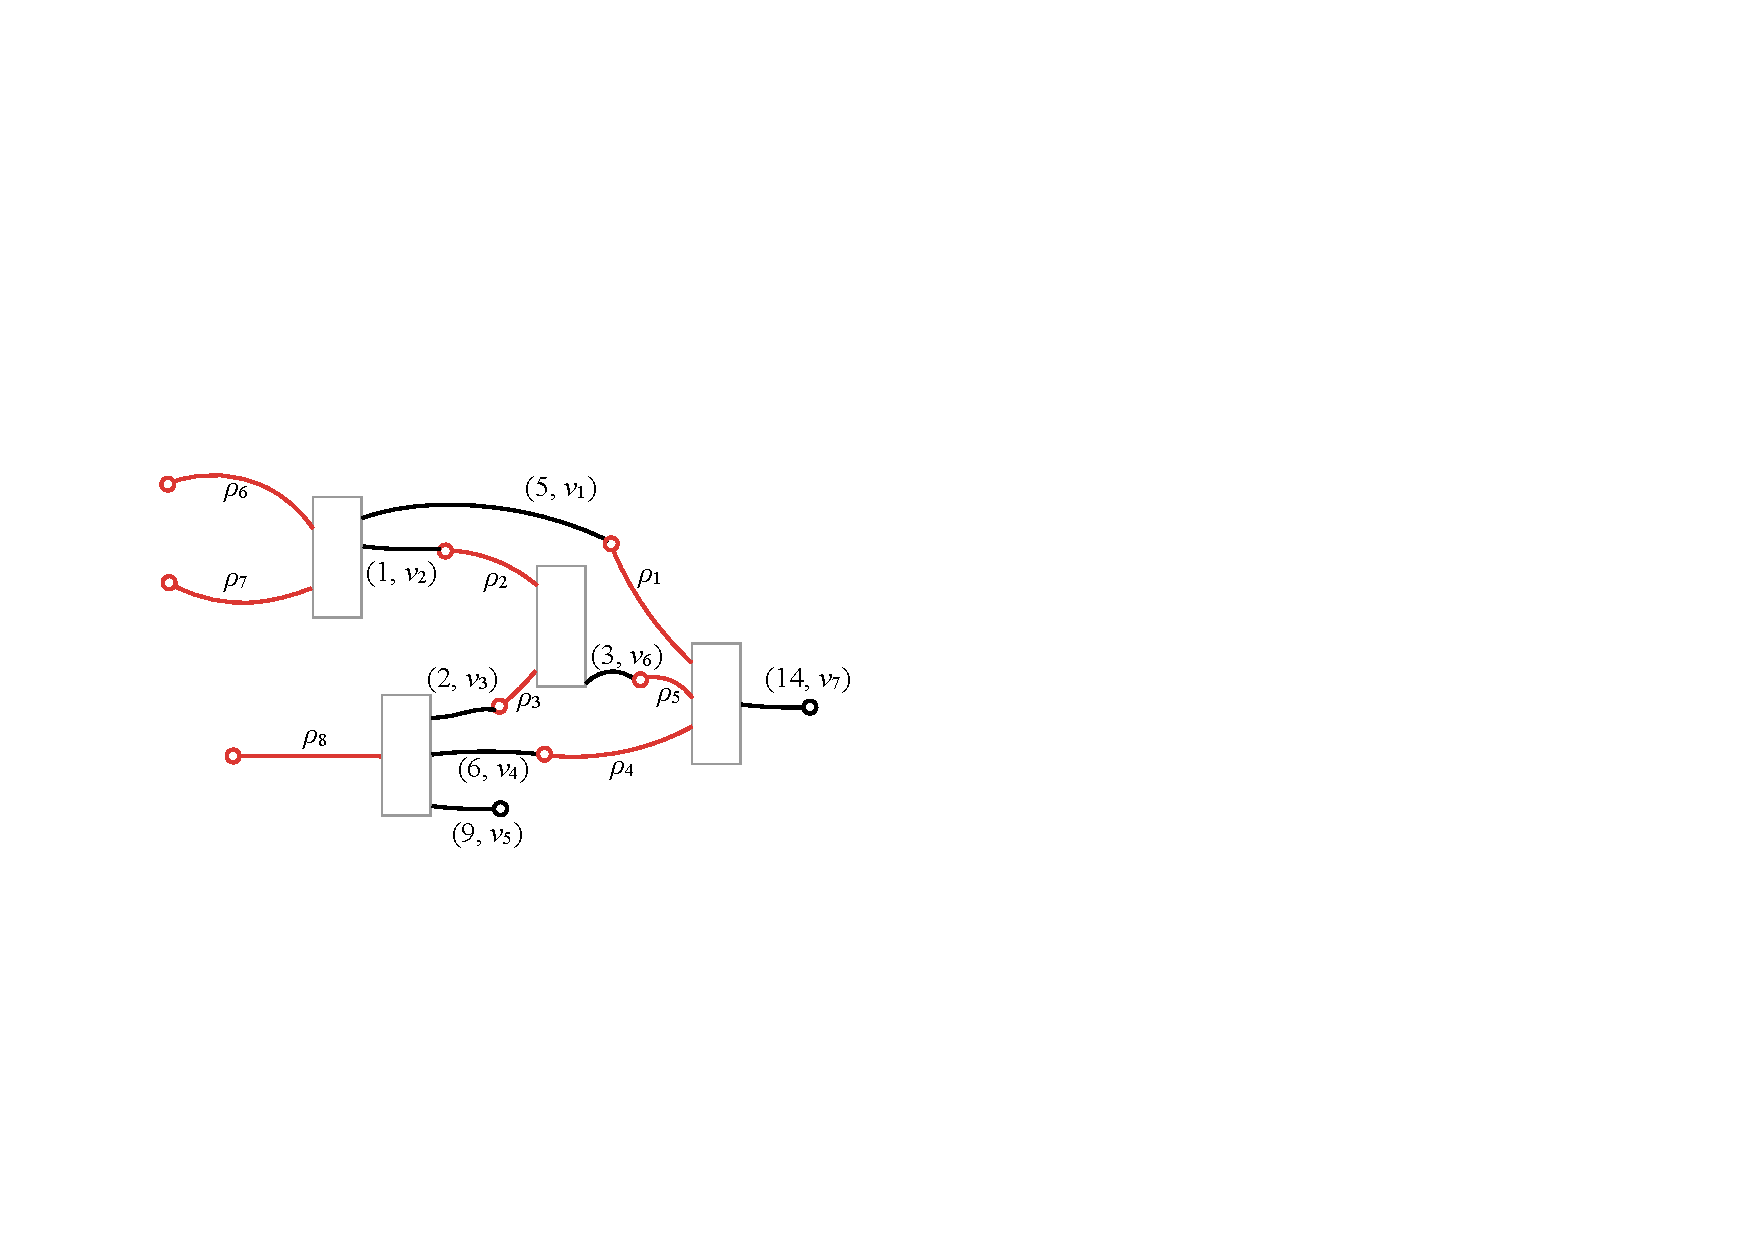
\includegraphics[width=\textwidth/2]{figures/utxo-graph.pdf}
 \caption{Example of a plain UTxO graph}
  \label{fig:utxo-graph}
\end{figure}


\begin{definition}[Value]

A \emph{value} $\mathsf{val}$ is a \emph{set} of \emph{tokens} represented as a triple $(\mathsf{pid} \rightarrow \mathsf{tok} \rightarrow q)$ where
\begin{itemize}
    \item $\mathsf{pid} \in \{0,1\}^k$ is the \emph{Minting Policy identifier}, an arbitrary string of bytes corresponding to the \emph{hash} of a corresponding \emph{Minting Policy script},
    \item $\mathsf{tok} \in \{0,1\}^k$ is the \emph{Token name}, an arbitrary string of bytes,
    \item $q \in \mathbb{Z}$ is the quantity of this particular token.
\end{itemize}

\end{definition}

We use $\mathsf{Val}$ to denote the set of all possible values and  $\mu_x$ for minting policy scripts.

\begin{definition}[Validator Script]
A validator script $\nu$ is a pure function whose type is:
\[
  \nu : (\delta : \txDataTy) \to (\rho : \txDataTy) \to (\mathsf{tx} : \txPendingTxTy)
  \to\txBoolTy,
\]
where: 
\begin{itemize}
    \item $\txDataTy$ is a universal data type, and we denote an empty value of type $\txDataTy$ by $\emptyset$,  
    \item $\delta$ is the \emph{datum} part of the output to which this particular script is locked (see Definition \ref{def:outputs}),
    \item $\rho$ is the \emph{redeemer} provided as part of the transaction being validated,
    \item $\txBoolTy = \{\bot, \top\},$
    \item $\txPendingTxTy$ is the \emph{validation context}.
\end{itemize}
\end{definition}

Validator scripts are called \emph{phase-2} scripts in the Alonzo Ledger specification (see \cite{alozon-spec} for a formal treatment of these). Informally, scripts are \emph{evaluated} by the ledger when it \emph{applies} a transaction to its current state to yield a new ledger state. Each validator script referenced by an output is passed its arguments drawn from the output it locks and the transaction context it is executed in. The transaction is valid if and only if all scripts evaluates to $\top.$

We denote by $V$ the set of all validator scripts.

\begin{definition}[Outputs]
\label{def:outputs}
An \emph{output} $o$ is a triple $\mathsf{Val} \times V \times \txDataTy.$
We denote by $O$ the set of all possible outputs, and by $O_x$ the outputs in some context $x$.
\end{definition}

\begin{definition}[Inputs]
An input $i$ is a pair $(\txOutRef, \rho)$ where 
$\txOutRef \in (\mathsf{TxId} \times \mathbb{N})$ is the input reference with $\mathsf{TxId} \subseteq \mathbb{B},$ and $\rho \in \txDataTy$ is the \emph{input}'s redeemer.  We denote by $I$ the set of all possible inputs, and by $I_x$ the outputs in some context $x$.
\end{definition}

\begin{definition}[Validation Context]

A validation context $\txPendingTx$ is a tuple  
$$(I_\sigma, O_\sigma, \mathsf{Mint}, \txRmin, \txRmax, \txKeys)$$
where:
\begin{itemize}
    \item $I_\sigma \in I^w$ is a list of inputs of length $w$,
    \item $O_\sigma \in O^y$ is a list of outputs of length $y$,
    \item $\mathsf{Mint} \subset \mathsf{Val}$ is the \emph{Minted} values,
    \item $(\txRmin, \txRmax) \in \mathcal{S} \times \mathcal{S}$ are the lower and upper validity bounds of the enclosing transaction, \todo{define time \& periods instead of slots}
    \item $\txKeys$ is the set of public keys signing the enclosing transaction.
\end{itemize}

\end{definition}

\subsection{State Machines}\label{sec:cem}
A convenient abstraction for EUTxO smart contracts spanning a sequence
of related transactions are state machines. Specifically, we adopt
\emph{constraint emitting machines (CEMs)}~\cite{eutxo}. These are
based on Mealy machines and consist of a set of states $\cemS$, a set
of inputs $\cemI$, a predicate \(\cemFinal : \cemS\to\txBoolTy\)
identifying final states, and a step relation
\(\cemStepRel{s}{i}{s'}{\cemTxCon}\), which takes a state $s$ on an
input $i$ to a successor state $s'$ under the requirements that the
constraints $\cemTxCon$ are satisfied.

We implement CEMs on a EUTxO ledger (the mainchain) by representing a sequence of CEM states as a sequence of transactions. Each of these transactions has got a \emph{state-machine input} $\cemIn$ and a \emph{state-machine output} $\cemOut$, where the latter is locked by a validator $\cemVal$, implementing the step relation. The only exceptions are the initial and final state, which have got no state-machine input and output, respectively.

\begin{figure}[t]
  \centering
  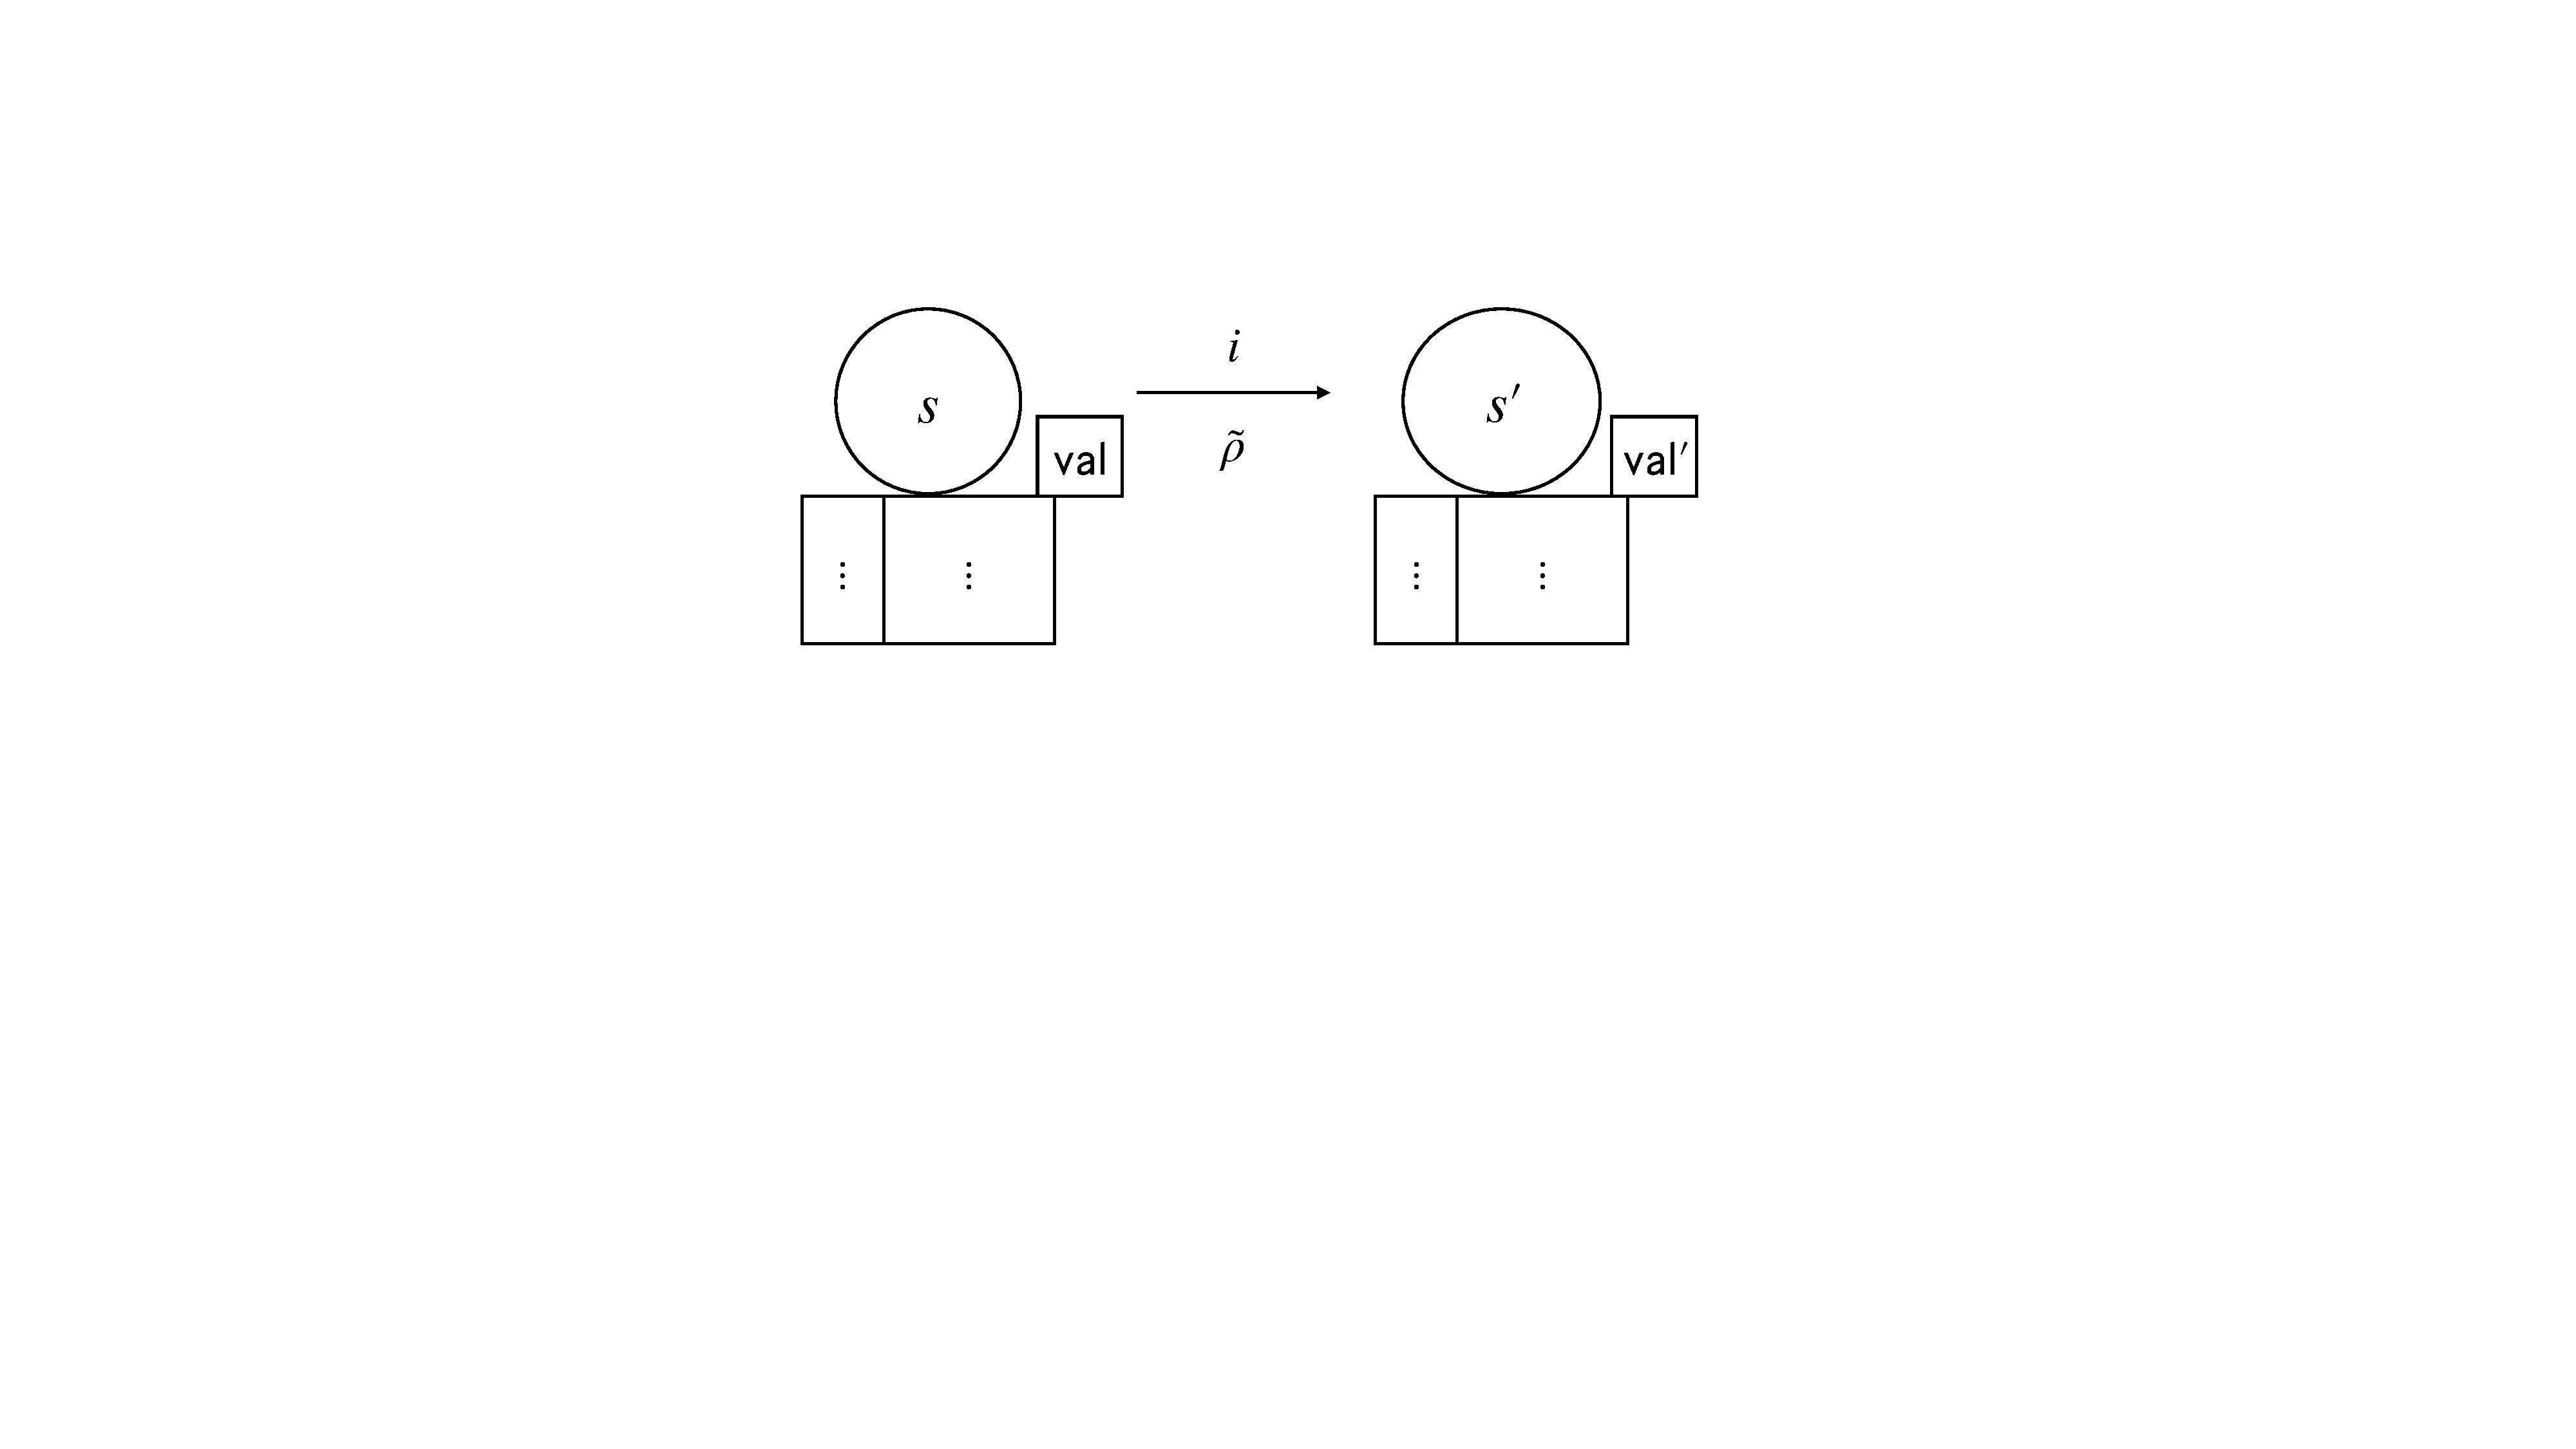
\includegraphics[scale=.2,width=\textwidth/2]{figures/state-transition_cropped.pdf}
  \caption{Transactions representing successive states in a CEM
    transition relation \(\cemStepRel{s}{i}{s'}{\cemTxCon}\).  Fields
    $\val$ and $\val'$ are the value fields of the state-machine
    outputs and $\tilde \rho$ is the additional data.}
  \label{fig:state-transition}
\end{figure}

More specifically, given two transactions $\tx$ and $\tx'$, they represent successive states under \(\cemStepRel{s}{i}{s'}{\cemTxCon}\) iff 

\begin{mitemize}
  \item state-machine output $\cemOut = (\txVal, \cemVal, s)$ of $\tx$
  is consumed by the state-machine input $\cemIn' = (\txOutRef, \rho)$
  of $\tx'$, whose redeemer is \(\rho = i\) (i.e., the redeemer
  provides the state-machine input) and
  \item either $\cemFinal(s') = \true$ and $tx'$ has no state-machine
  output, or $\cemOut' = (\txVal', \cemVal, s')$ and $\tx'$ meets all
  constraints imposed by $\cemTxCon$.
\end{mitemize}
Sometimes it is useful to have additional data $\tilde \rho$ provided
as part of the redeemer, i.e., $\rho = (i,\tilde \rho)$.

A state transition of the described type is represented by two connected
transactions as shown in Fig.~\ref{fig:state-transition}.  For
simplicity, state-machine inputs and outputs are not shown, with the
exception of the value fields $\txVal$ and $\txVal'$ of the state-machine output.


%%% Local Variables:
%%% mode: latex
%%% TeX-master: "main"
%%% End:


\section{Protocol Overview}\label{sec:overview}

\todo{maybe change terminology (mainchain -> L1, offchain -> L2)}

The Hydra Head protocol provides functionality to lock a set of UTxOs on a
blockchain, referred to as the \emph{mainchain}, and evolve it inside a
so-called offchain \emph{head}, independently of the mainchain. At any point,
the head can be closed with the effect that the locked set of UTxOs on the
mainchain is replaced by the latest set of UTxOs inside the head. The protocol
guarantees full wealth preservation: no generation of funds can happen offchain
(inside a head) and no responsive honest party involved in a head can ever lose
any funds other than by consenting to give them away. In exchange for decreased
liveness guarantees (stop any time), it can essentially proceed at network speed
under good conditions, thereby reducing latency and increasing throughput in an
optimal way. At the same time, the head protocol provides the same capabilities
as the mainchain by reusing the same ledger model and transaction formats --- it's
isomorphic.

\subsection{Opening the head}

To create a head-protocol instance, any party may take the role of an
\emph{initiator} and ask other parties, the \emph{head members}, to participate
in the head by exchanging public keys and agreeing on other protocol parameters.
This public-key material is used both for the authentication of head-related
onchain transactions that are restricted to head members (e.g., a non-member is
not allowed to close the head) and for multisignature-based event confirmation
in the head.

The initiator then establishes the head by submitting an \emph{initial}
transaction to the mainchain that contains the head parameters and mints special
\emph{participation tokens (PT)} identifying the head members. The
\emph{initial} transaction also initializes a state machine (see
Fig.~\ref{fig:SM_states_basic}) that manages the ``transfer'' of UTxOs into the
head and back. The state machine comprises the four states $\stInitial$,
$\stOpen$, $\stClosed$, and $\stFinal$. A \emph{state thread token (ST)} minted
in \emph{initial} marks the head output and ensures contract
continuity~\cite{eutxo}.

\begin{figure}[t!]
  \centering
  \begin{tikzpicture}[>=stealth,auto,node distance=2.8cm, initial text=$\mathsf{init}$, every
    state/.style={text width=10mm, text height=2mm, align=center}]
    \node[state, initial] (initial) {$\stInitial$};
    \node[state] (open) [above right of=initial] {$\stOpen$};
    \node[state] (closed) [right of=open] {$\stClosed$};
    \node[state] (final) [below right of=closed] {$\stFinal$};

    \path[->] (initial) edge [bend left=20] node {$\stCollect$} (open);
    \path[->] (open) edge [bend left=20] node {$\stClose$} (closed);
    \path[->] (closed) edge [bend left=20] node {$\stFanout$} (final);
    \path[->] (closed) edge [loop above] node {$\stContest$} (closed);
    \path[->] (initial) edge node {$\stAbort$} (final);
  \end{tikzpicture}

  \caption{Mainchain state diagram for this version of the Hydra protocol.}\label{fig:SM_states_basic}
\end{figure}

%%% Local Variables:
%%% mode: latex
%%% TeX-master: "main"
%%% End:


Once the initial transaction appears on the mainchain, establishing the initial
state $\stInitial$, each head member can attach a \mtxCom{} transaction, which
locks (on the mainchain) the UTxOs that the party wants to commit to the head.

The commit transactions are subsequently collected by the \mtxCCom{} transaction
causing a transition from $\stInitial$ to $\stOpen$. Once the $\stOpen$ state is
confirmed, the head members start running the off-chain \emph{head protocol},
which evolves the initial UTxO set (the union over all UTxOs committed by all
head members) independently of the mainchain. For the case where some head
members fail to post a \mtxCom{} transaction, the head can be aborted by going
directly from $\stInitial$ to $\stFinal$.

\subsection{The Coordinated Head protocol}

The actual Head protocol starts after the initialization phase with an initial
set of UTxOs that is identical to the UTxOs locked onchain via the \mtxCom{}
and \mtxCCom{} transactions.

The protocol distributes and \emph{collects} individual transactions in full
concurrency off-chain, while each party maintains their view of the local UTxO
state. That is, the current set of UTxOs evolved from the initial UTxO set by
applying transactions as they are received from the other parties.

To confirm transactions and allow for an onchain decommit of the resulting UTxO
set without needing the whole transaction history, UTxO snapshots
$\Uset_1,\Uset_2,\ldots$ are created. The first snapshot corresponds to the
initial UTxO set and snapshots have a strict sequence.

For this, a \emph{snapshot leader} requests his view of a new confirmed state to
be multisigned as a new snapshot. The leader does not need to send his local
state, but only indicate, by hashes, the set of transactions to be included in
order to obtain the to-be-snapshotted UTxO set.

The other participants sign the snapshot as soon as they have (also) seen the
transactions that are to be processed on top of its preceding snapshot: a
party's local state is always ahead of the latest confirmed snapshot.

Signatures are broadcast and aggregated by each party. When all signature parts
of the multi-signature are received and verified, a snapshot is considered
confirmed. As a consequence, a participant can safely delete (if wished) all
transactions that have been processed into it as the snapshot's multisignature
is now evidence that this state once existed during the head evolution.

\subsection{Closing the head}

The head protocol is designed to allow any head member at any point in time to
produce, without interaction, a certificate for the current head UTxO set. This
certificate is created from the latest confirmed snapshot, specifically from its
snapshot number and the respective multisignature. Using this certificate, the
head member may ``force close'' the head by advancing the mainchain state
machine to the $\stClosed$ state.

Once in $\stClosed$, the state machine grants parties a \emph{contestation
  period}, during which each party may (one single time) contest the closure by
providing the certificate for a newer head UTxO set. Contesting leads back to
the state $\stClosed$. After the contestation period has elapsed, the state
machine may proceed to the $\stFinal$ state. The state machine enforces that the
outputs of the transaction leading to $\stFinal$ correspond exactly to the
latest UTxO set seen during the contestation period.

\subsection{Differences}

In the Coordinated Head protocol, off-chain consensus is simplified by not having transactions
confirmed concurrently to the snapshots (and to each other) but having the snapshot leader propose,
in their snapshot, a set of transactions for explicit confirmation. The parties' views of confirmed
transactions thus progress in sync with each other (once per confirmed snapshot), thus simplifying
the close/contest procedure on the mainchain. Also, there is no need for conflict resolution as
in Appendix~B of~\cite{hydrahead20}. In summary, the differences to the original Head protocol in~\cite{hydrahead20} are:

\begin{itemize}
  \item No hanging transactions due to `coordination'.
  \item No acknowledgement nor confirmation of transactions.
  \item No confirmation of snapshots (two-round confirmation by local acknowledgement).
\end{itemize}
\todo{explain why?}

%%% Local Variables:
%%% mode: latex
%%% TeX-master: "main"
%%% End:


\section{Protocol Setup}\label{sec:setup}
In order to create a head-protocol instance, an initiator invites a set of
participants (the initiator being one of them) to join by announcing to them the
protocol parameters.

\begin{itemize}
  \item For onchain transaction authentication (Cardano) purposes, each party $\party_i$ generates a
        corresponding key pair $(\msVK_{i},\msSK_{i})$ and sends their verification key $\msVK_{i}$ to all other parties. In the case of Cardano, these are Ed25519 keys.

  \item For offchain signing (Hydra) purposes, a very basic multisignature scheme (MS, as defined in Section~\ref{sec:multisig}) based on EdDSA using Ed25519 keys is used:
        \begin{itemize}
          \item $\msKeyGen$ is Ed25519 key generation (requires no parameters)
          \item $\msSign$ creates an EdDSA signature
          \item $\msCombVK$ is concatenation of verification keys into an ordered list
          \item $\msComb$ is concatenation of signatures into an ordered list
          \item $\msVfy$ verifies the "aggregate" signature by verifying each individual EdDSA signature under the corresponding Ed25519 verification key
        \end{itemize}\todo{Move this and previous bullet point into the preliminary section}
        
  \item Each party $\party_i$ generates a hydra key pair and sends their hydra verification key to all other parties.

  \item Each party $\party_i$ computes the aggregate key from the received verification keys, stores the aggregate key,
        their signing key as well as the number of participants $\nop$.
        
  \item Each party establishes pairwise communication channels to all other parties. That is, every network message received from a specific party is checked for (channel) authentication. It is the implementer’s duty to find a suitable authentication process for the communication channels.
  
  \item All parties agree on a contestation period $\cPer$.
\end{itemize}

If any of the above fails (or the party does not agree to join the head in the
first place), the party aborts the initiation protocol and ignores any further
action. Finally, at least one of the participants posts the \mtxInit{} transaction
onchain as described next in Section~\ref{sec:on-chain}.

%%% Local Variables:
%%% mode: latex
%%% TeX-master: "main"
%%% End:


% TODO: Provided by researchers (keep up-to-date)
% Taken from: paper-hydra/engineering/coordinatedhead
\section{On-chain Protocol}\label{sec:on-chain}

\todo{Problem: Always ensure abort is possible. E.g. by individual aborts!?}

We describe the details of the \emph{on-chain} protocol controlling a
Hydra head (see Fig.~\ref{fig:SM_states_basic}) using the CEM abstraction \&
notation (see Section~\ref{sec:cem}). In addition of standard CEM modeling, we
also provide the formal conditions $\cemTxCon$ which a transition need to
satisfy and also include them in the accompanying text.

The following sections describe the structure of each of the transactions
comprising the Head protocol: $\mtxInit{}$, $\mtxCom{}$, $\mtxAbort{}$,
$\mtxCollect{}$, $\mtxClose{}$, $\mtxContest{}$, and $\mtxFanout{}$. Following
the EUTxO model, this structure is enforced on-chain through \emph{validators}
which are \emph{scripts instances} attached to each UTxO and run as part of the
ledger's validation of the transaction (see Section~\ref{sec:eutxo}). The
protocol defines one minting policy script and three validator scripts:
\begin{itemize}
  \item $\muHead$ governs the minting of state and participation tokens,
  \item $\nuInitial$ controls initialization and how UTxOs are committed to the head, while
  \item $\nuCommit$ controls the collection of committed UTxOs into the head, and lastly
  \item $\nuHead$ controls the main protocol state-machine logic.
\end{itemize}

\subsection{Init transaction}

The \mtxInit{} transaction creates a head instance and establishes the initial
state of the protocol and is shown in Figure~\ref{fig:SM_commit_tx}. The head
instance is represented by the unique\footnote{As the EUTxO ledger preventing
  double-spending, the uniqueness of $\cid$ is guaranteed because $i_{seed}$ can
  only be spent once} currency identifier $\cid$ created by minting tokens using
the parameterized $\muHead$ minting policy script:
\[
  \cid = \hash(\muHead(i_{seed}))
\]
\noindent where $i_{seed} \in \txInputs$ is a transaction input and the
$\muHead(i_{seed})$ minting policy validator checks:
\begin{menumerate}
  \item $i_{seed}$ is spent in this transaction
  $i_{seed} \in \txInputs$\todo{Only when minting, allow burning always}
\end{menumerate}

\vspace{0.1cm}
\noindent Two kinds of tokens are minted:
\begin{itemize}
  \item A single \emph{State Thread (ST)} token marking the output carrying the state
        of the protocol on-chain, whose name is the well known string
        \texttt{HydraHeadV1}, i.e.
        $\st = (\cid \rightarrow \texttt{HydraHeadV1} \rightarrow 1)$\todo{$\st = (\cid \rightarrow \texttt{HydraHeadV1}$}
  \item One \emph{Participation Token (PT)} per participant
        $i \in \{1 \dots \nop \}$, where the token name is the participant's
        verification key hash $\keyHash_{i}$, i.e.
        $\pt_{i} = (\cid \rightarrow \keyHash_{i} \rightarrow 1)$.\todo{$\pt = (\cid \rightarrow \keyHash_{i})$}
\end{itemize}

\noindent Consequently, the \mtxInit{} transaction

\begin{itemize}
  \item has at least input $i_{seed}$,
  \item mints one $\st$ and one $\pt$ for each of the $\nop$ participants with
        policy $\cid :: \{\st, \pt_{1}, \ldots, \pt_{\nop}\}$,
  \item has one state-machine output locked by $\nuHead$ with datum
        $\datum_{\mathsf{head}}$
  \item has $\nop$ outputs, where each output is locked by $\nuInitial$ and the
        $\ith i$ output has the participation token $\pt_i$ in its value, and
        $\cid$ as datum.
\end{itemize}

\noindent The initial state of the protocol is captured in the state-machine output datum
\[
  \datum_{\mathsf{head}} = (\stInitial,\cid,\hpAK,\hppuv,\nop,\cPer)
\]\todo{Explicitly NOT include $\hppuv$! as it is not guaranteed on-chain to be consistent with PTs}
where
\begin{mitemize}
  \item $\stInitial$ is a state identifier,
  \item $\cid$ is the unique currency id of this instance,
  \item $\hpAK$ is the aggregated off-chain multi-signature key established during the
  setup phase,
  \item $\hppuv$ is the list of all participants verification keys
  $(k_1,\ldots,k_\nop)$ exchanged during the setup phase and identifying the
  head members on-chain,
  \item $\nop$ is the number of head participants, and
  \item $\cPer$ is the length of the contestation period.
\end{mitemize}

\noindent Validator $\nuInitial$ ensures that the output is consumed by either
an \mtxAbort{}~\ref{sec:abort-tx} or a \mtxCom{}~\ref{sec:commit-tx}
transaction. Note that the general well-formedness and validity of the
\mtxInit{} transaction is checked on the mainchain, but head members need to
additionally check whether the initial state has the right $\cid$ and is
consistent with parameters agreed during setup.

\begin{figure}[h]

  \centering

  % 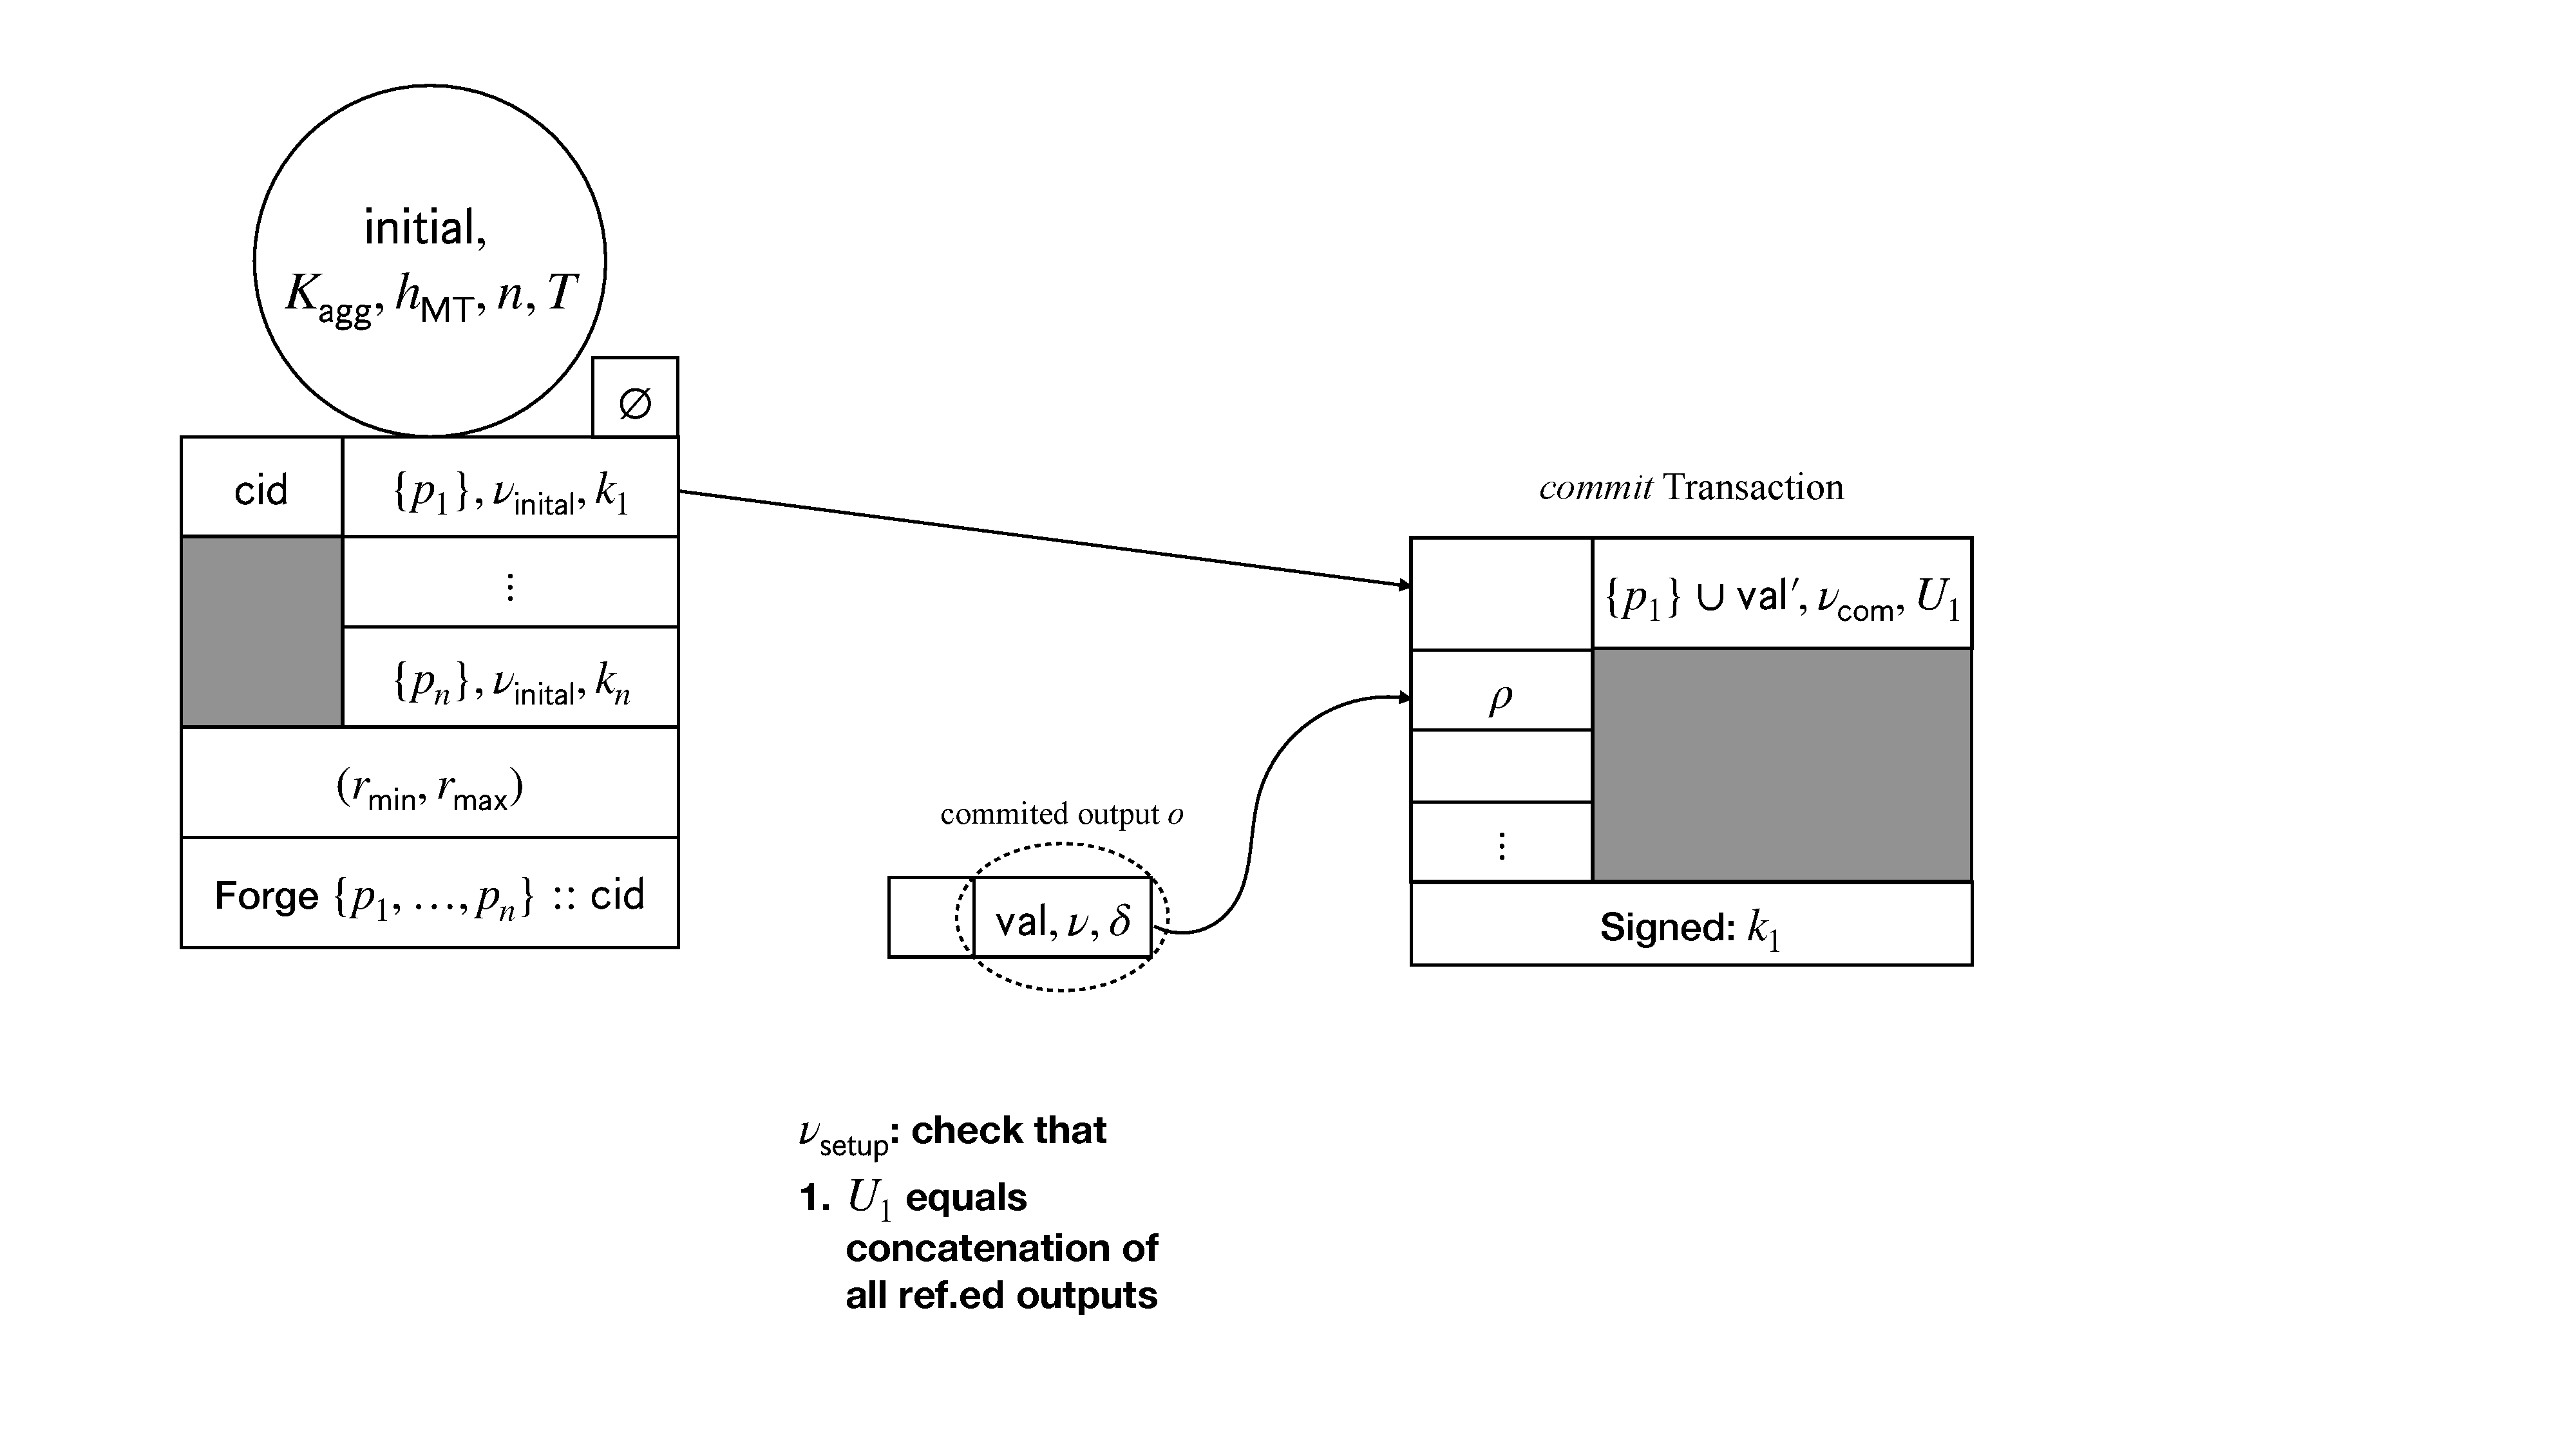
\includegraphics[width=\textwidth/2,trim=130 330 430 50,clip]{figures/SM_commit_tx.pdf}

  % TODO: clean draw marked up version
  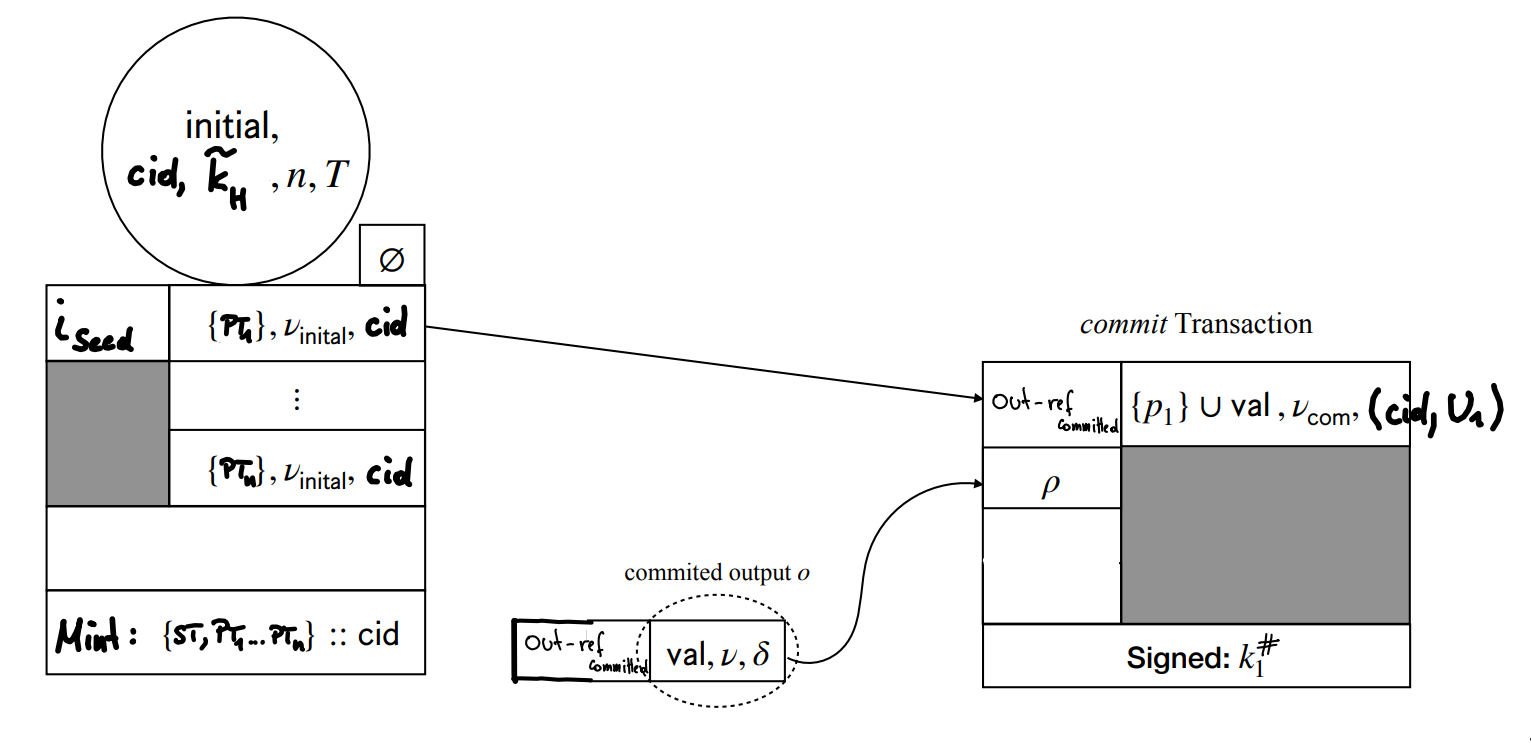
\includegraphics[width=\textwidth*2/3]{figures/SM_commit_tx.png}

  \caption{
    \mtxInit{} transaction (left) with one \mtxCom{} transaction
    (right) attached locking one output (center).}\label{fig:SM_commit_tx}

\end{figure}


%%% Local Variables:
%%% mode: latex
%%% TeX-master: "main"
%%% End:


\subsection{Commit Transaction}\label{sec:commit-tx}

A \mtxCom{} transaction may be submitted by each participant
$\forall i \in \{1 \dots \nop\}$ and is depicted on the right hand side of
Figure~\ref{fig:SM_commit_tx}. It has the following structure:
\begin{itemize}
  \item One input $i_{initial} = (\txOutRef_{initial}, \redeemer_{initial})$
        spending $o_{initial} = (\val_{initial}, \nuInitial, \datum_{initial})$
  \item Zero or one input with reference $\txOutRef_{commit}$ spending output
        $o_{committed} = (\val_{committed}, \cdot , \cdot)$
  \item One output $o_{commit} = (\val_{commit}, \nuCommit, \delta_{commit})$\todo{need to check output address?}
\end{itemize}

\noindent The $\nuInitial$ validator ensures that:
\begin{menumerate}
  \item The initial datum provides the currency id $\cid = \datum_{initial}$
  \item The initial redeemer references the committed output $\redeemer_{initial} = \txOutRef_{committed}$
  \item The committed value is in the output $\val_{com} = \val_{initial} \cup \val_{committed}$
  \item The currencty id and committed output are recorded in the output datum
  $\delta_{commit} = (\cid, U_{i})$ where
  $U_{i} = (\txOutRef_{committed},\bytes(o_{committed}))$
  \item Transaction is signed by a participant $\exists (\cid \rightarrow \keyHash_{i} \rightarrow 1) \in \val_{commit} \Rightarrow \keyHash_{i} \in \txKeys$
  \todo{need to check against head datum ($\hppuv$)?}
  \item No minting or burning  $\txMint = \varnothing$
\end{menumerate}

\noindent The $\nuCommit$ validator ensures the output is collected by either a \mtxCCom{}~\ref{sec:collect-tx} or \mtxAbort{}~\ref{sec:abort-tx} transaction of the on-chain state machine, selected by the appropriate redeemer.

\subsection{CollectCom Transaction}\label{sec:collect-tx}

\begin{figure}[h]

  \centering

  % 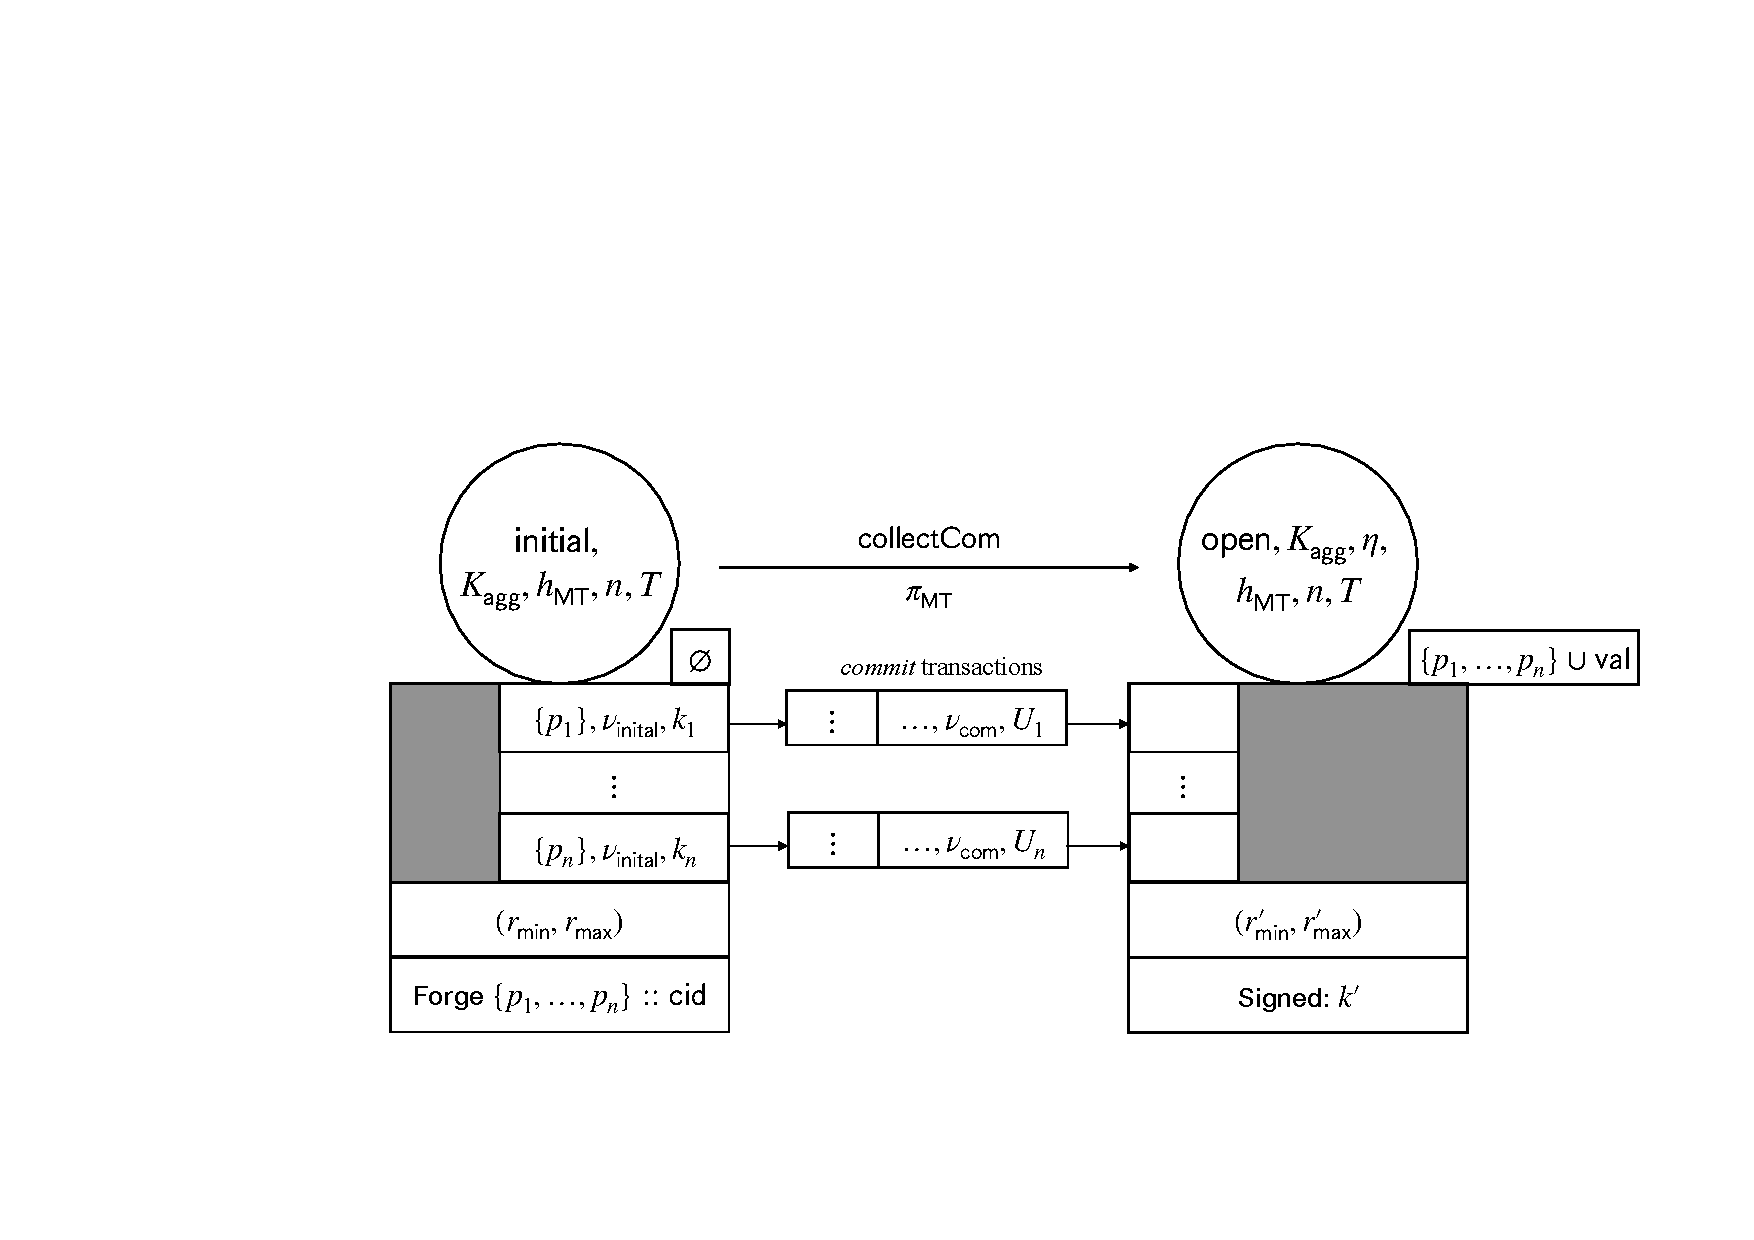
\includegraphics[width=\textwidth/2]{figures/SM_initial_open.pdf}
  %
  % TODO: clean draw marked up version
  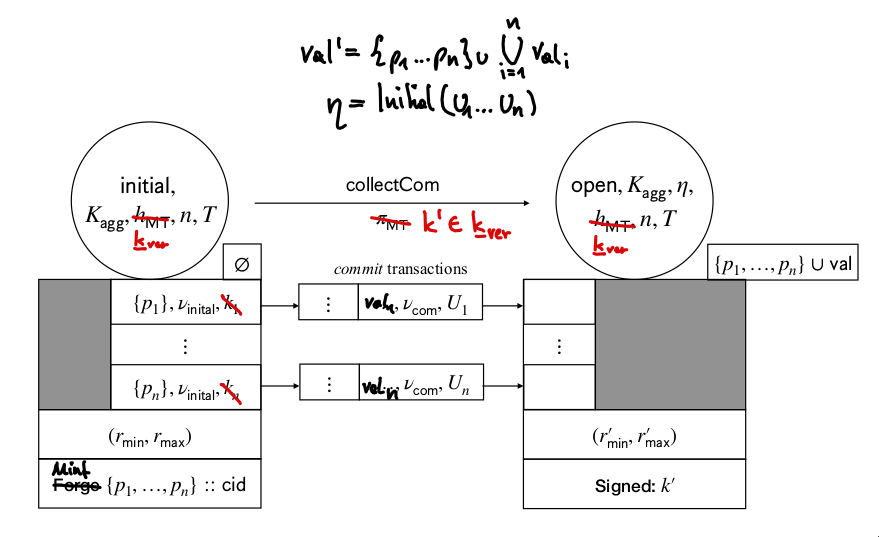
\includegraphics[width=\textwidth/2]{figures/SM_initial_open.png}

  \caption{\mtxInit{} transaction (left) with \mtxCCom{} transaction
    (right) and \mtxCom{} transactions (center).}
  \label{fig:SM_initial_open}

\end{figure}



%%% Local Variables:
%%% mode: latex
%%% TeX-master: "main"
%%% End:


\noindent The \mtxCCom{} transaction collects all the committed UTxOs to the same head. It has
\begin{itemize}
  \item one input spending from $\nuHead$ holding the $\st$, and
  \item $\forall i \in \{1 \dots \nop\}$ inputs spending \mtxCom{} outputs $(\val_{commit_i}, \nuCommit, (\cid, U_{i}))$ with $\pt_{i} \in \val_{commit_{i}}$.
\end{itemize}
The input spending from and paying to the $\nuHead$ validator, checks the state
of the CEM is advanced:
\[
   (\stInitial,\cid,\hpAK,\hppuv,\nop,\cPer) \xrightarrow{\mathsf{collectCom}} (\stOpen,\cid,\hpAK,\hppuv,\nop,\cPer,\eta)
\]

\noindent Furthermore, $\nuHead$ checks these constraints:
\begin{menumerate}
  \item Collect commits in $\eta = (0, U^{\#})$ as the hash, of the concatenation, of
  the serialised representation of committed outputs $U_{i}$, which are sorted by their associated $\txOutRef$\footnote{Sorting is required to ensure a canonical representation which can also be reproduced from the UTxO set later in the fanout.}: \todo{sortByOutRef
    not defined, needed?} \todo{is this clear enough?}
  \[
    \underline{U}_{sorted} = \mathsf{sortByOutRef} ( U_{1}, \dots, U_{\nop} )
  \]
  \[
    U^{\#} = \hash(\bigoplus_{\forall (\cdot, b_{j})~\in~\underline{U}_{sorted}} b_{j}))
  \]
  \item All committed value captured and no additional funds ``enter'' or ``leave''\\
  $\val' = \mathsf{ST} \cup (\bigcup_{i=1}^{n} \val_{commit_i})$
  \item All tokens present in output\footnote{This is sufficient as a Head participant would check off-chain whether a Head is initialized correctly with the right number of tokens.}
  $|\{\cid \rightarrow . \rightarrow 1\} \in \val'| = \nop + 1$\todo{notation? enumerate $\pt_{i}$ using $\hppuv$ instead?}
  \item Transaction is signed by a participant $\exists (\cid \rightarrow \keyHash_{i} \rightarrow 1) \in \val_{commit} \Rightarrow \keyHash_{i} \in \txKeys$\todo{also check $\keyHash_{i} \in \hppuv$?}
  \item Unchanged parameters $\cid$, $\hpAK$, $\hppuv$, $\nop$, and
  $\cPer$ \todo{explicitly state this?}
  \item No minting or burning  $\txMint = \varnothing$
\end{menumerate}

\noindent Each spent $\nuCommit$ validator ensures that:
\begin{menumerate}
  \item The ST token is present in the output value
  $\st = (\cid \rightarrow ``HydraHeadV1'' \rightarrow 1) \in \val'$, where
  $(\cid,\cdot) = \delta_{commit}$ is given by the datum of the commit output
  $o_{commit}$.
\end{menumerate}

\subsection{Abort Transaction}\label{sec:abort-tx}

\begin{figure}

  \centering

  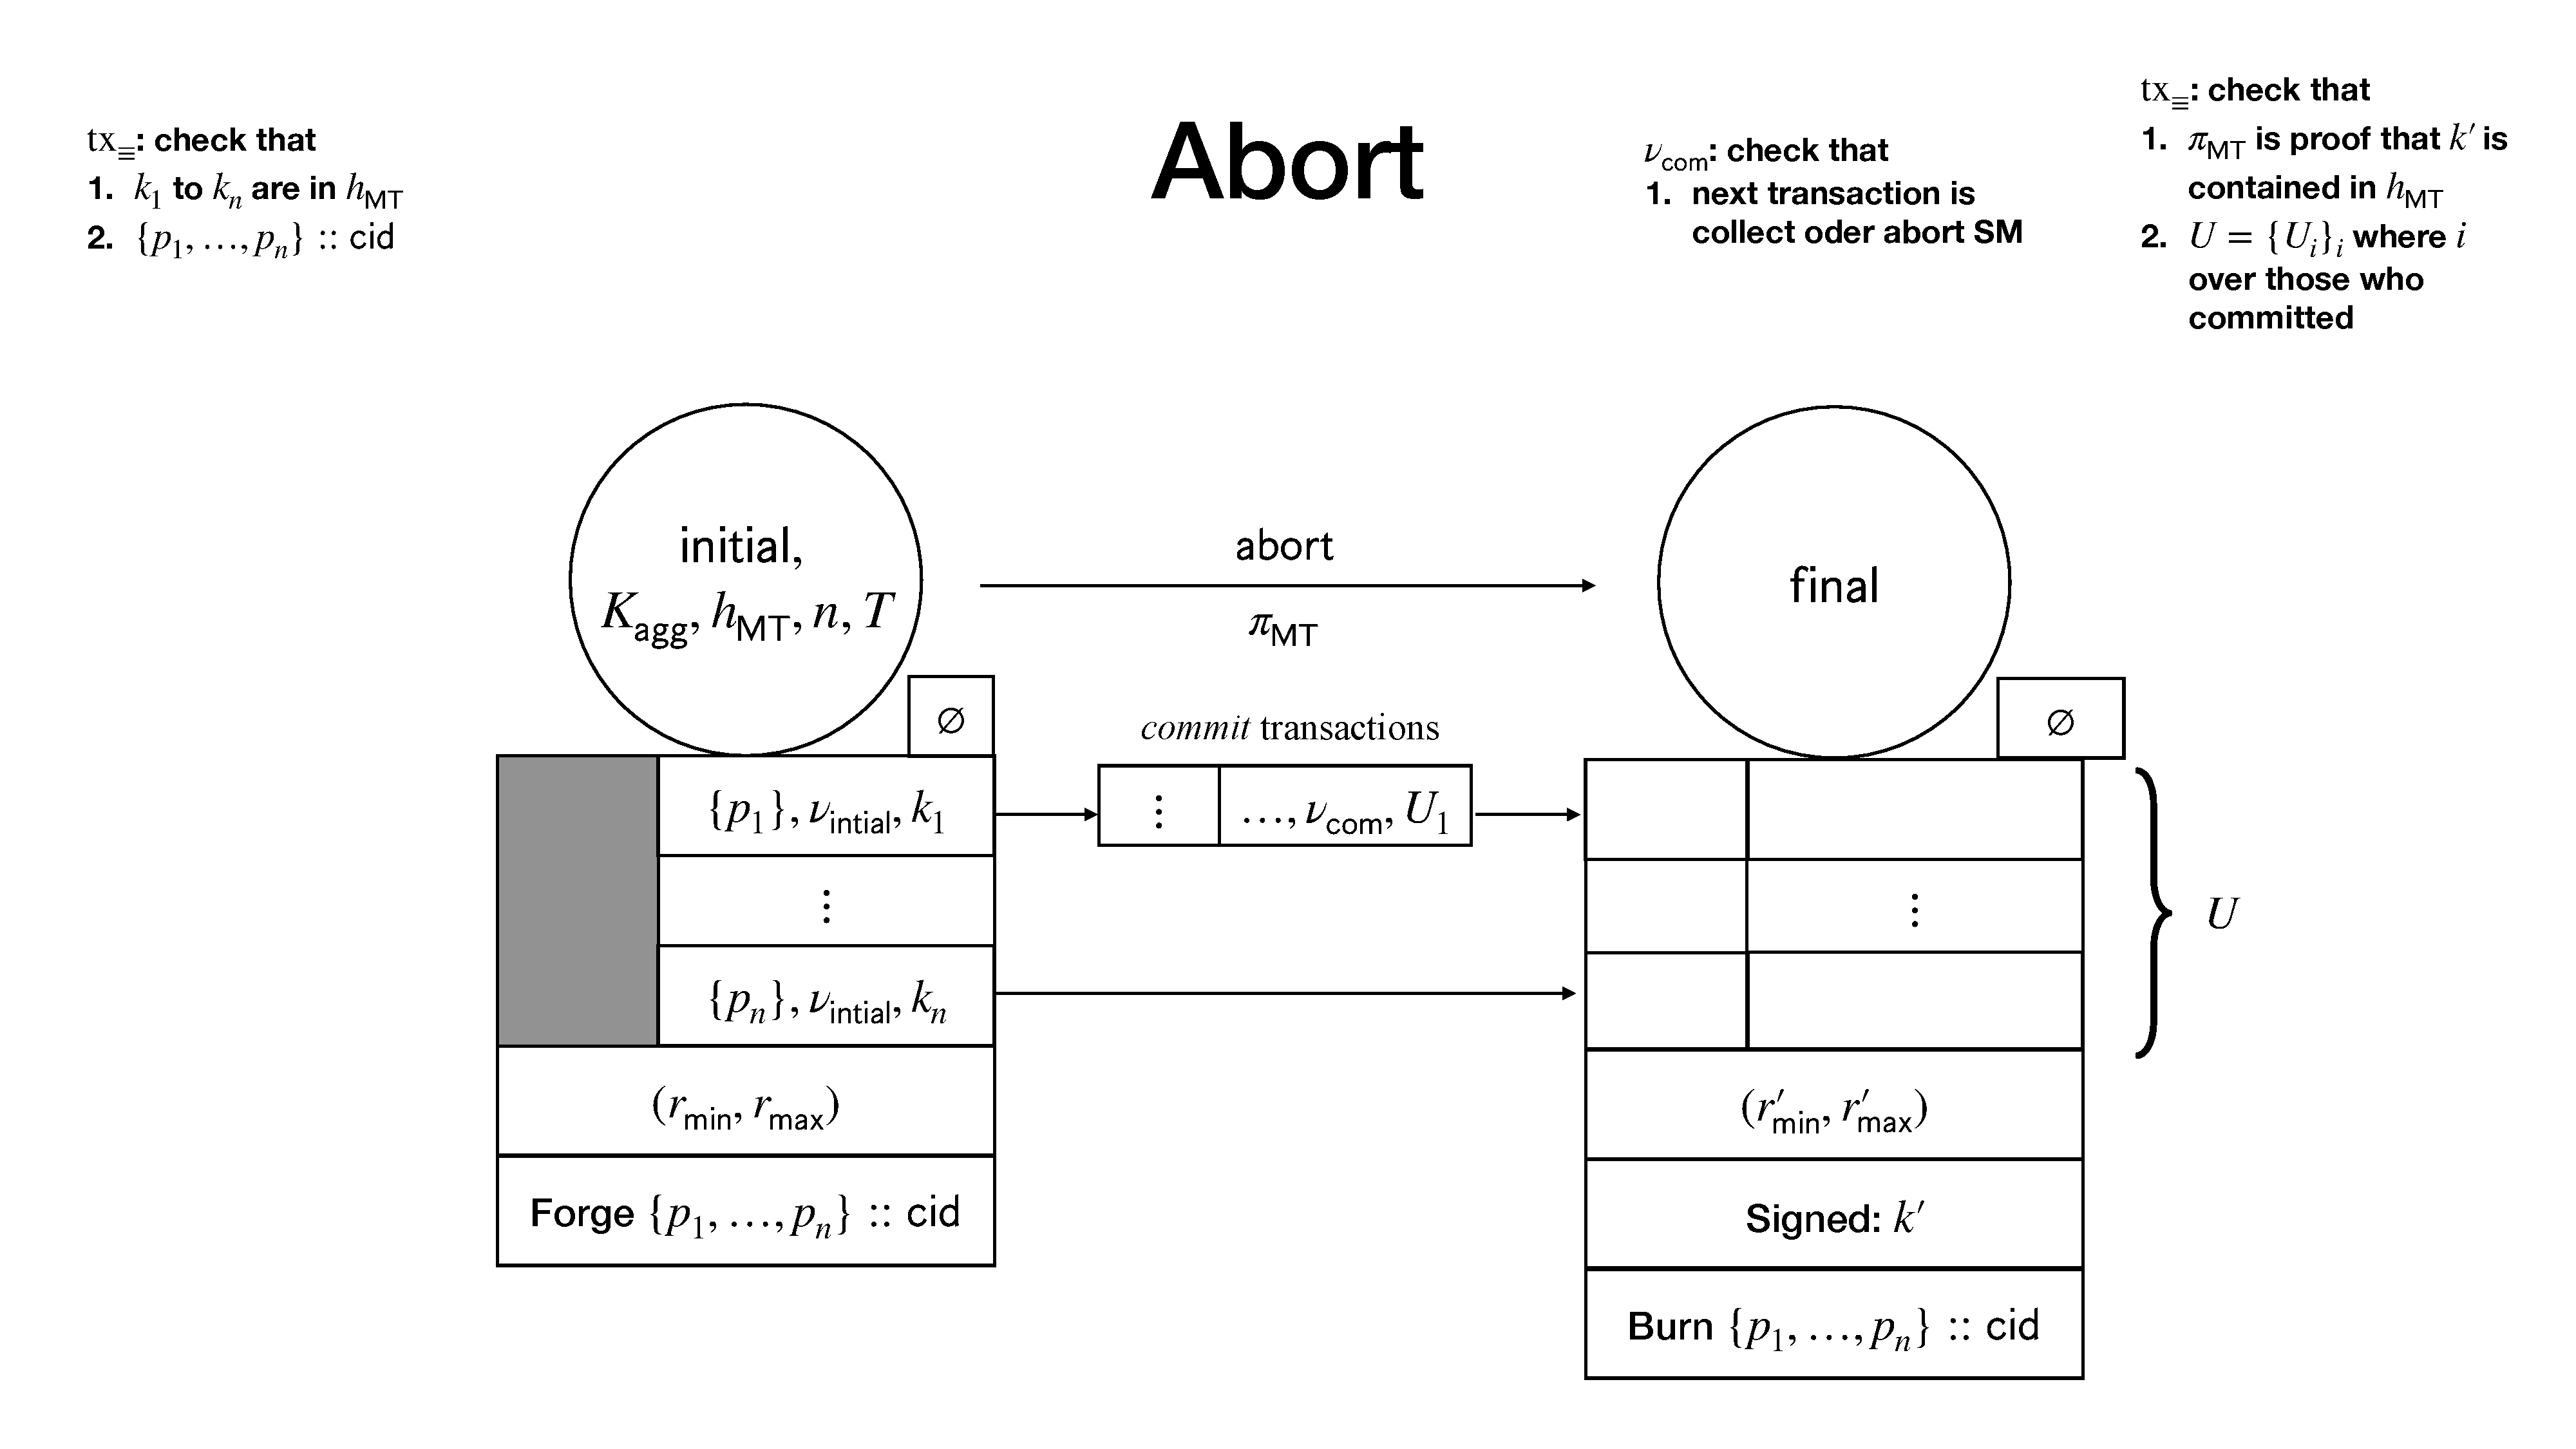
\includegraphics[width=\textwidth/2-2em,trim=350 20 240 300,
  clip]{figures/SM_initial_final.pdf}
    
  \caption{\mtxInit{} transaction (left) with \mtxAbort{} transaction
    (right) and \mtxCom{} transactions (center).}
  \label{fig:SM_initial_final}

\end{figure}



%%% Local Variables:
%%% mode: latex
%%% TeX-master: "main"
%%% End:


The \mtxAbort{} transaction (see Figure~\ref{fig:SM_initial_final}) allows a
party to abort the creation of a head. It is comprised of
\begin{itemize}
  \item one input spending from $\nuHead$ holding the $\st$, and
  \item $\forall i \in \{1 \dots \nop\}$ inputs either
    \begin{itemize}
      \item spending from an initial output $(\val_{initial_i}, \nuInitial, \cid)$ with $\pt_{i} \in \val_{initial_i}$, or
      \item spending from a commit output $(\val_{commit_i}, \nuCommit, \datum_{commit_i})$ with $\pt_{i} \in \val_{commit_{i}}$,\todo{detail datums below?}
    \end{itemize}
  \item $m$ outputs to redistribute already committed UTxOs.
\end{itemize}
Note that \mtxAbort{} represents a final transition of the CEM and hence there
is no state machine output. The input spending from $\nuHead$ does provide the
number of reimbursed outputs $m$ as redeemer and checks the state of the CEM is
advanced to the final $\stFinal$ as follows:

\[
   (\stInitial,\cid,\hpAK,\hppuv,\nop,\cPer) \xrightarrow[m]{\mathsf{abort}} \stFinal.
\]

\noindent The $\nuHead$ validator ensures that:
\begin{menumerate}
  \item All UTxOs committed into the head are reimbursed exactly as they were
  committed. By comparing hashes of serialised representations of the $m$
  reimbursing outputs\footnote{Only the first $m$ outputs are used for
    reimbursing, while more outputs may be present in the transaction, e.g for
    change} and canonically sorted (by $\txOutRef$) committed UTxOs $U_{i}$ where $(\cdot, U_{i}) = \datum_{commit_{i}}$ from \mtxCom{}~\ref{sec:commit-tx}:
  \todo{list/tuple comprehensions?}
  \[
    \underline{U}_{sorted} = \mathsf{sortByOutRef} ( \forall i \in \{1\dots\nop\} : U_{i} \neq \bot => U_{i})
  \]
  \[
    \hash(\bigoplus_{j}{\underline{U}_{sorted}[j]}^{\downarrow 2}) = \hash(\bigoplus_{j=1}^{m} \bytes(\txOutputs[j]))
  \]

  \item Transaction is signed by a participant $\exists (\cid \rightarrow \keyHash_{i} \rightarrow -1) \in \txMint \Rightarrow \keyHash_{i} \in \txKeys$
  \item All tokens are burnt
  $|\{\cid \rightarrow \cdot \rightarrow -1\} \in \txMint| = n + 1$\todo{number
    of tokens burned vs. explicit enumeration what to burn?}
\end{menumerate} 

\noindent Each $\nuInitial$ validator checks:\todo{datums/redeemers here?}
\begin{menumerate}
  \item The ST is getting burned
  $(\cid \rightarrow \texttt{HydraHeadV1} \rightarrow -1) \subseteq \txMint$,
  where $\cid$ is given by the datum of the spent initial output
  $\cid = \delta_{initial}$.
\end{menumerate}

\noindent Each $\nuCommit$ validators checks:
\begin{menumerate}
  \item The ST is getting burned
  $(\cid \rightarrow \texttt{HydraHeadV1} \rightarrow -1) \subseteq \txMint$,
  where $\cid$ is given by the datum of the spent commit output $(\cid,\cdot) = \delta_{commit}$.
\end{menumerate}

\subsection{Close Transaction}\label{sec:close-tx}

\begin{figure}[t!]

  \centering

  %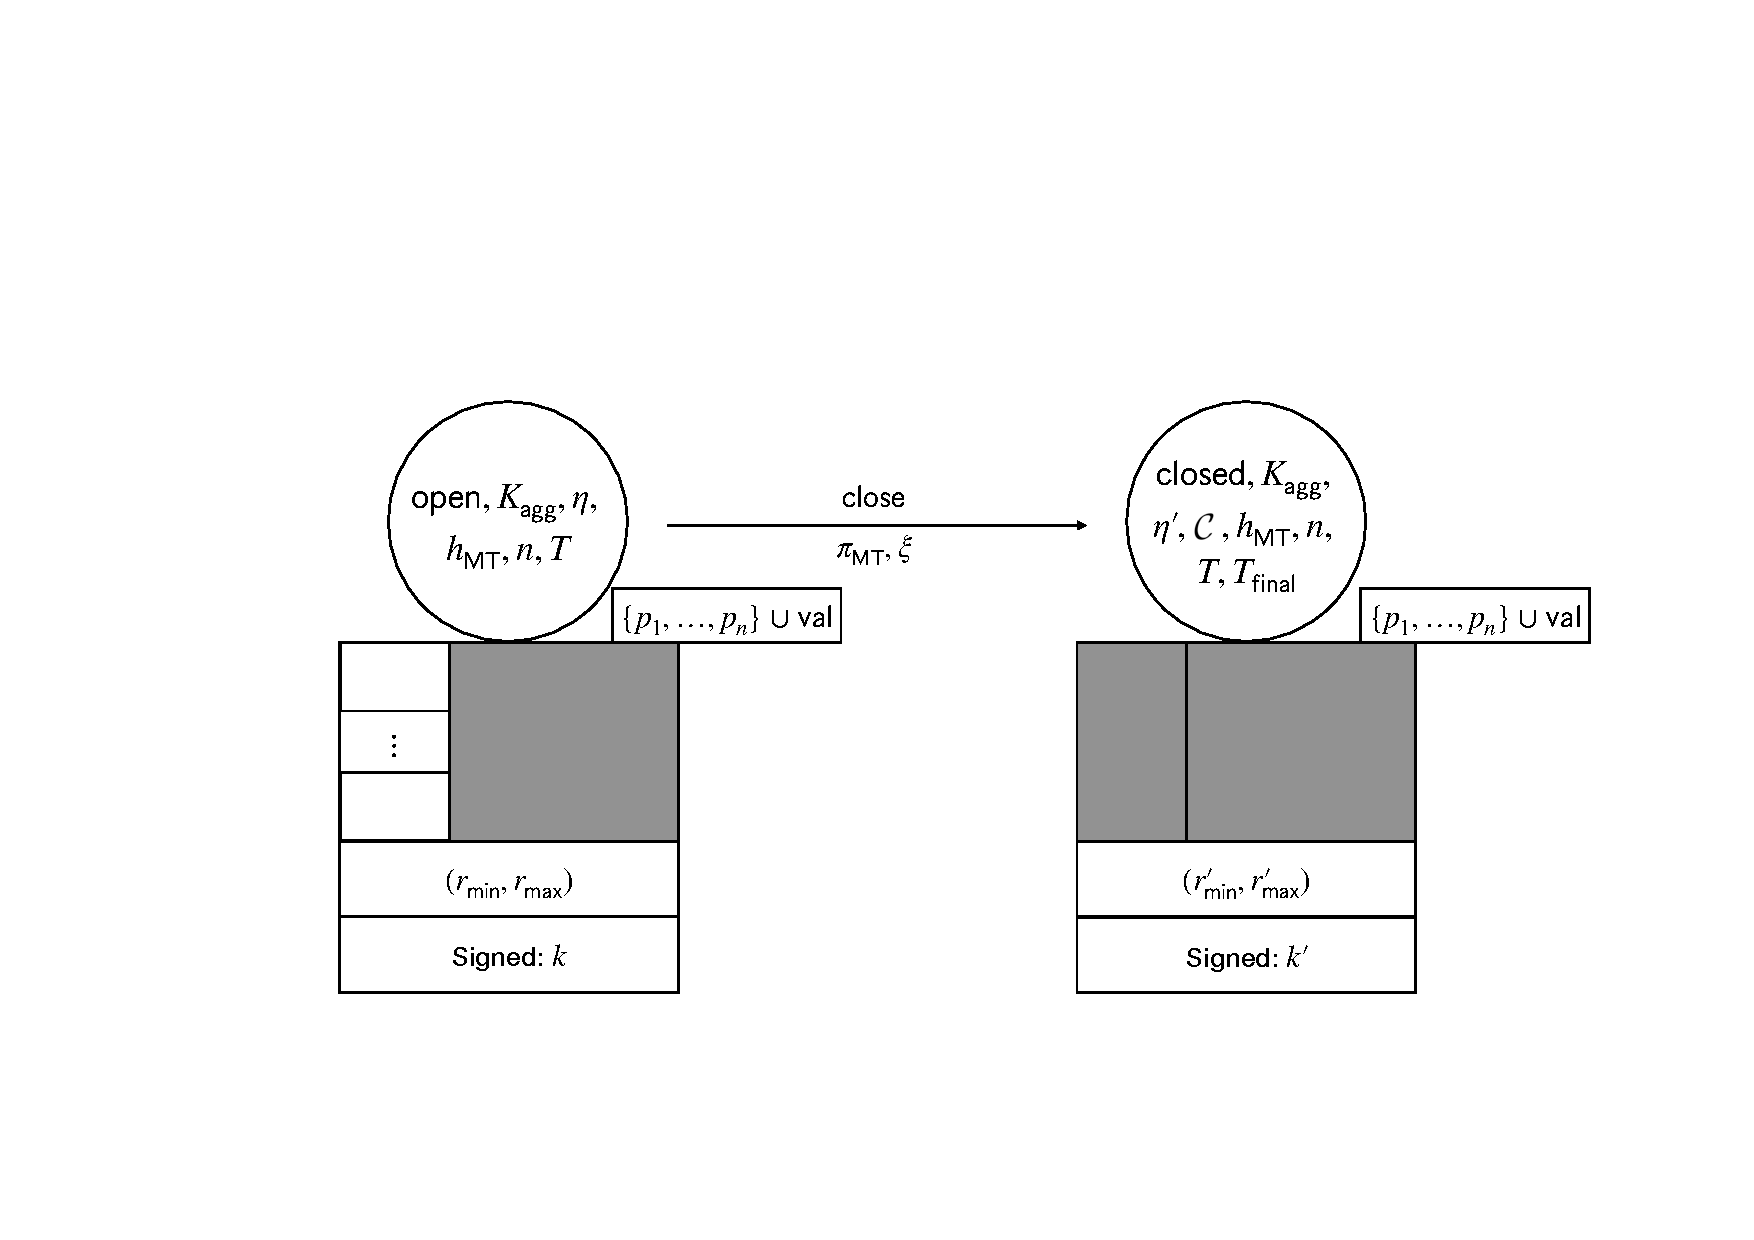
\includegraphics[width=\textwidth/2-2em,trim=350 100 160 300,
  %clip]{figures/SM_open_closed.pdf}

  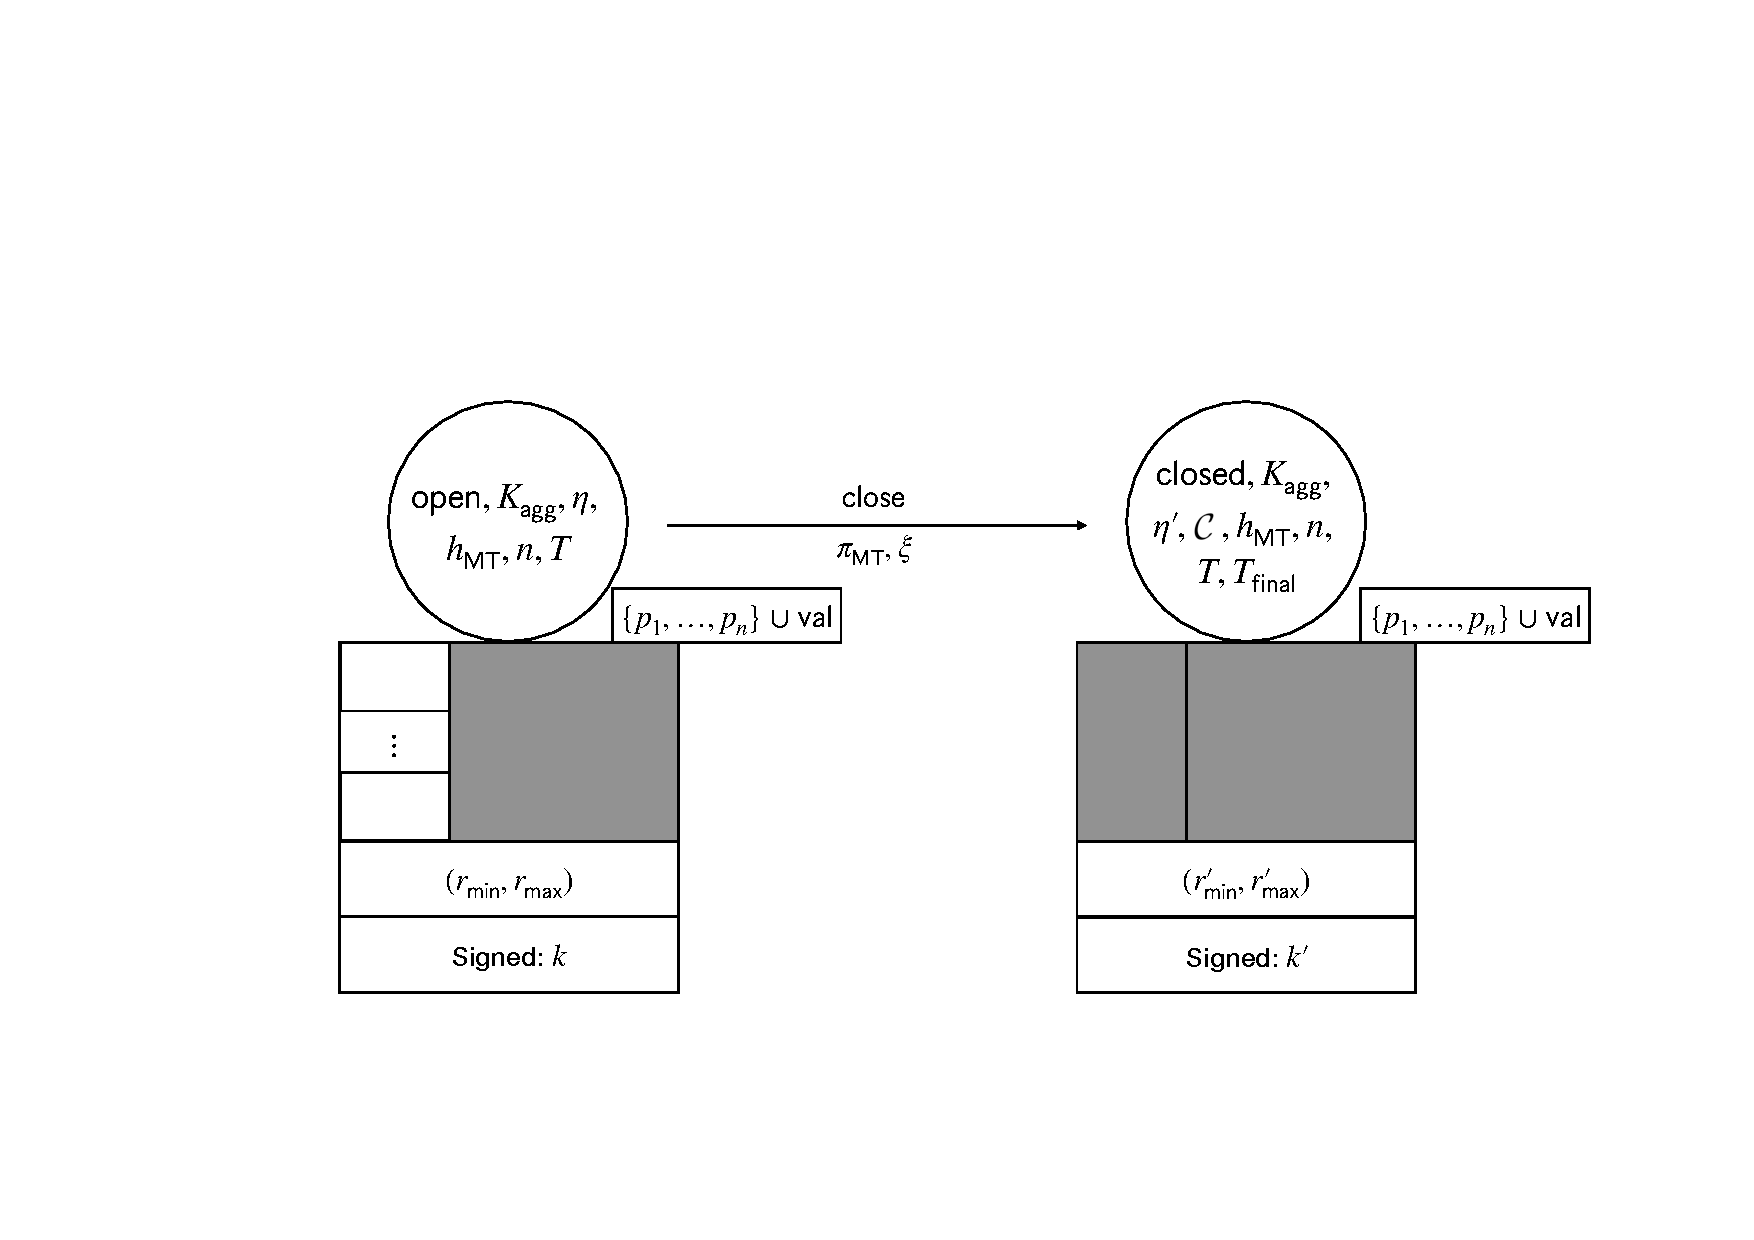
\includegraphics[width=\textwidth/2]{figures/SM_open_closed.pdf}

  \caption{\mtxCCom{} transaction (left) with \mtxClose{}
    transaction (right).}
  \label{fig:SM_open_closed}

\end{figure}



%%% Local Variables:
%%% mode: latex
%%% TeX-master: "main"
%%% End:


In order to close a head, a head member may post the \mtxClose{} transaction
(see Figure~\ref{fig:SM_open_closed}). This transaction has a single input
spending from the $\nuHead$ and paying to the $\nuHead$ validator, which checks
the state of the CEM is advanced:
\[
  (\stOpen,\cid,\hpAK,\hppuv,\nop,\cPer,\eta) \xrightarrow[\xi]{\mathsf{close}} (\stClosed,\cid,\hpAK,\hppuv,\nop,\cPer,\eta_0,\eta',\contesters,\Tfinal)
\]

\noindent The $\nuHead$ validator performs these checks:
\begin{enumerate}
  \item Recorded the initial snapshot state $\eta_0 = \eta$
  \item New snapshot state $(s', \cdot) = \eta'$ is the initial $\eta_{0}$
        or correctly signed via $\xi$ \\
        \[
          \left\{\begin{array}{ll}
                  \msVfy(\hpAK,(\cid || \eta_{0} || \eta'),\xi) = \true & \mathrm{if} ~ s' > 0, \\
                  \eta' = \eta_{0} & \mathrm{otherwise}
                 \end{array}\right.
        \]\todo{factor out $s'$?}
  \item Initialize the set of contesters\footnote{This allows the closing party
        to also contest and is required for use cases where pre-signed, valid in
        the future, close transactions are used to delegate head closing}
        $\contesters = \emptyset$
  \item Correct contestation deadline $\Tfinal = \txRmax + T$
  \item Bounded confirmation window\footnote{Ensures head $\Tfinal$ is at most
        $2*T$ in the future} $\txRmax - \txRmin \leq T$
  \item Value in the head is preserved $\val' = \val$
  \item Transaction is signed by a participant $\exists (\cid \rightarrow \keyHash_{i} \rightarrow 1) \in \val' \Rightarrow \keyHash_{i} \in \txKeys$
  \item No minting or burning $\txMint = \varnothing$
\end{enumerate}

\subsection{Contest Transaction}\label{sec:contest-tx}

\begin{figure}

  \centering

  %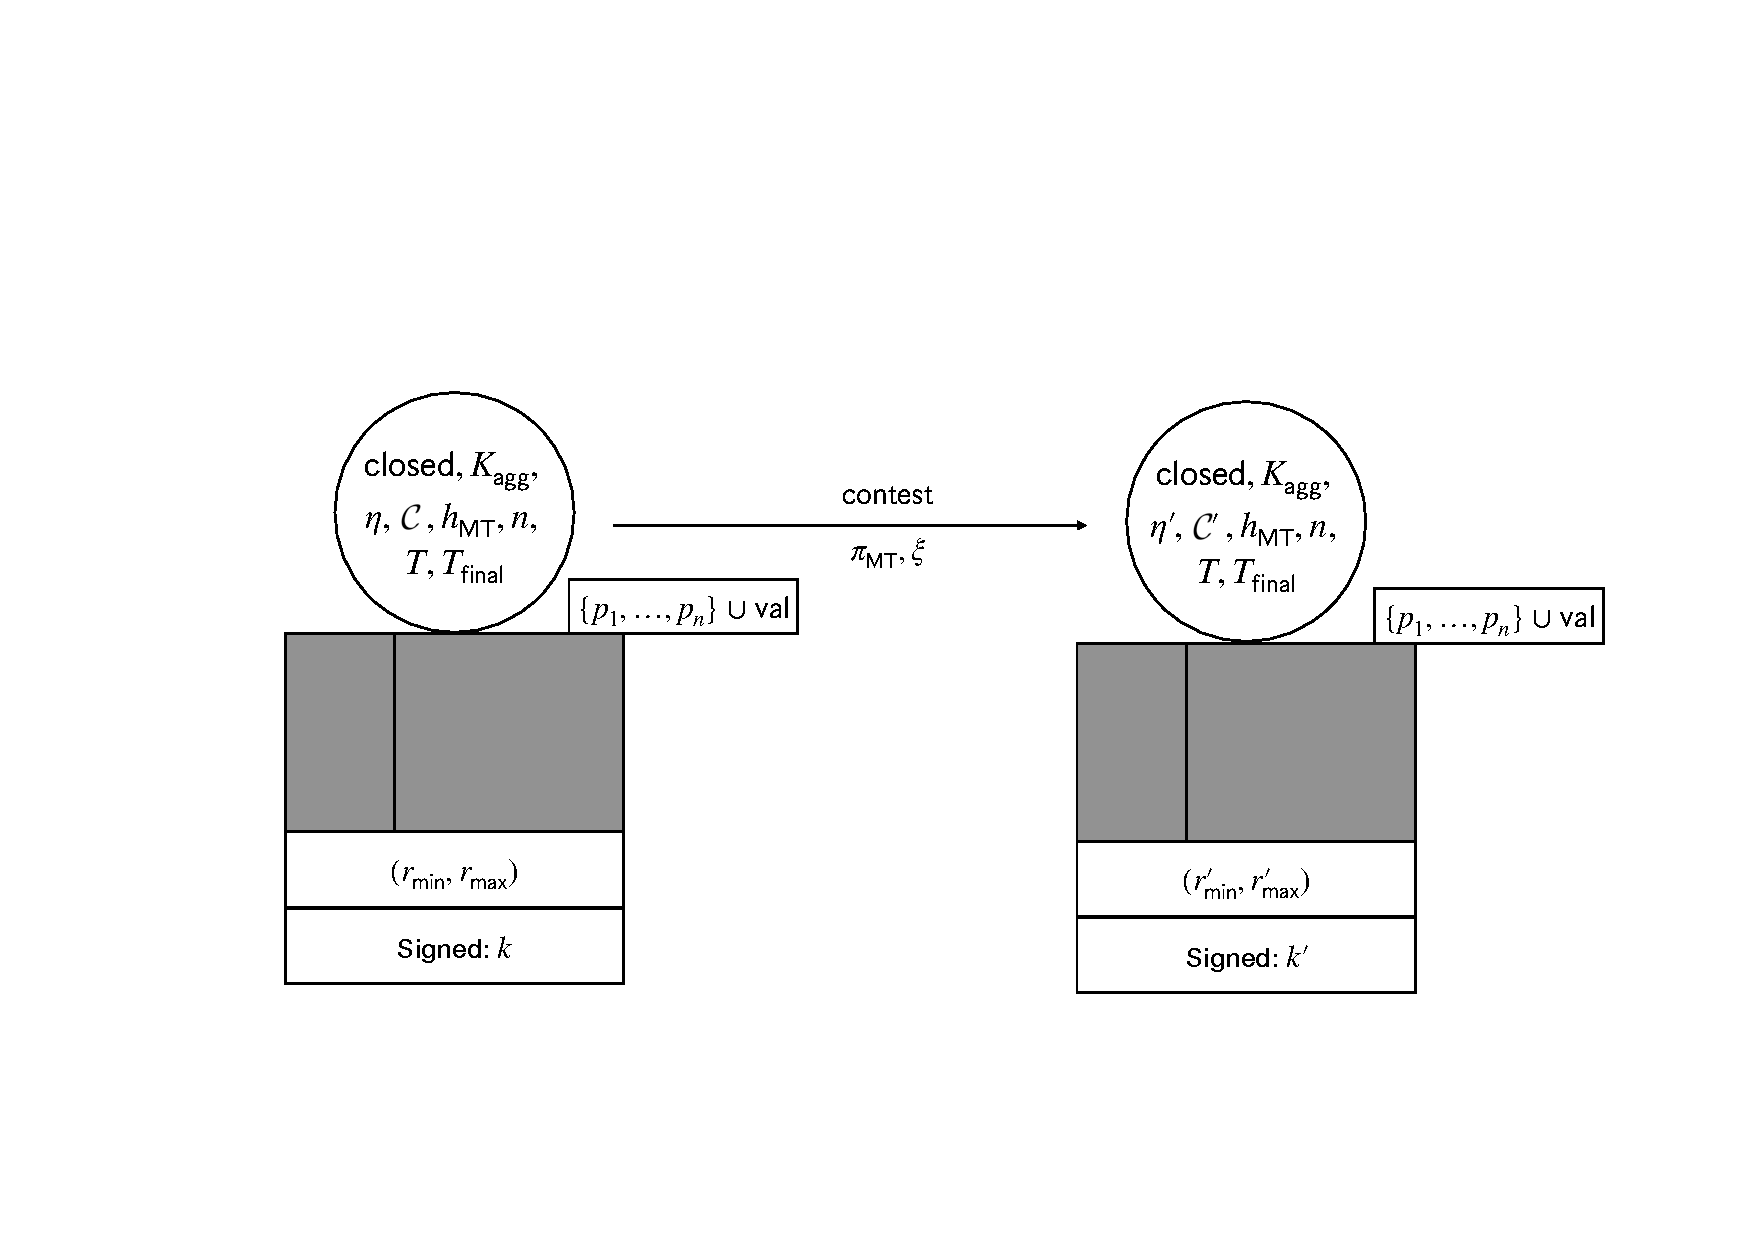
\includegraphics[width=\textwidth/2-2em,trim=280 120 160 260,
  %clip]{figures/SM_closed_closed.pdf}

  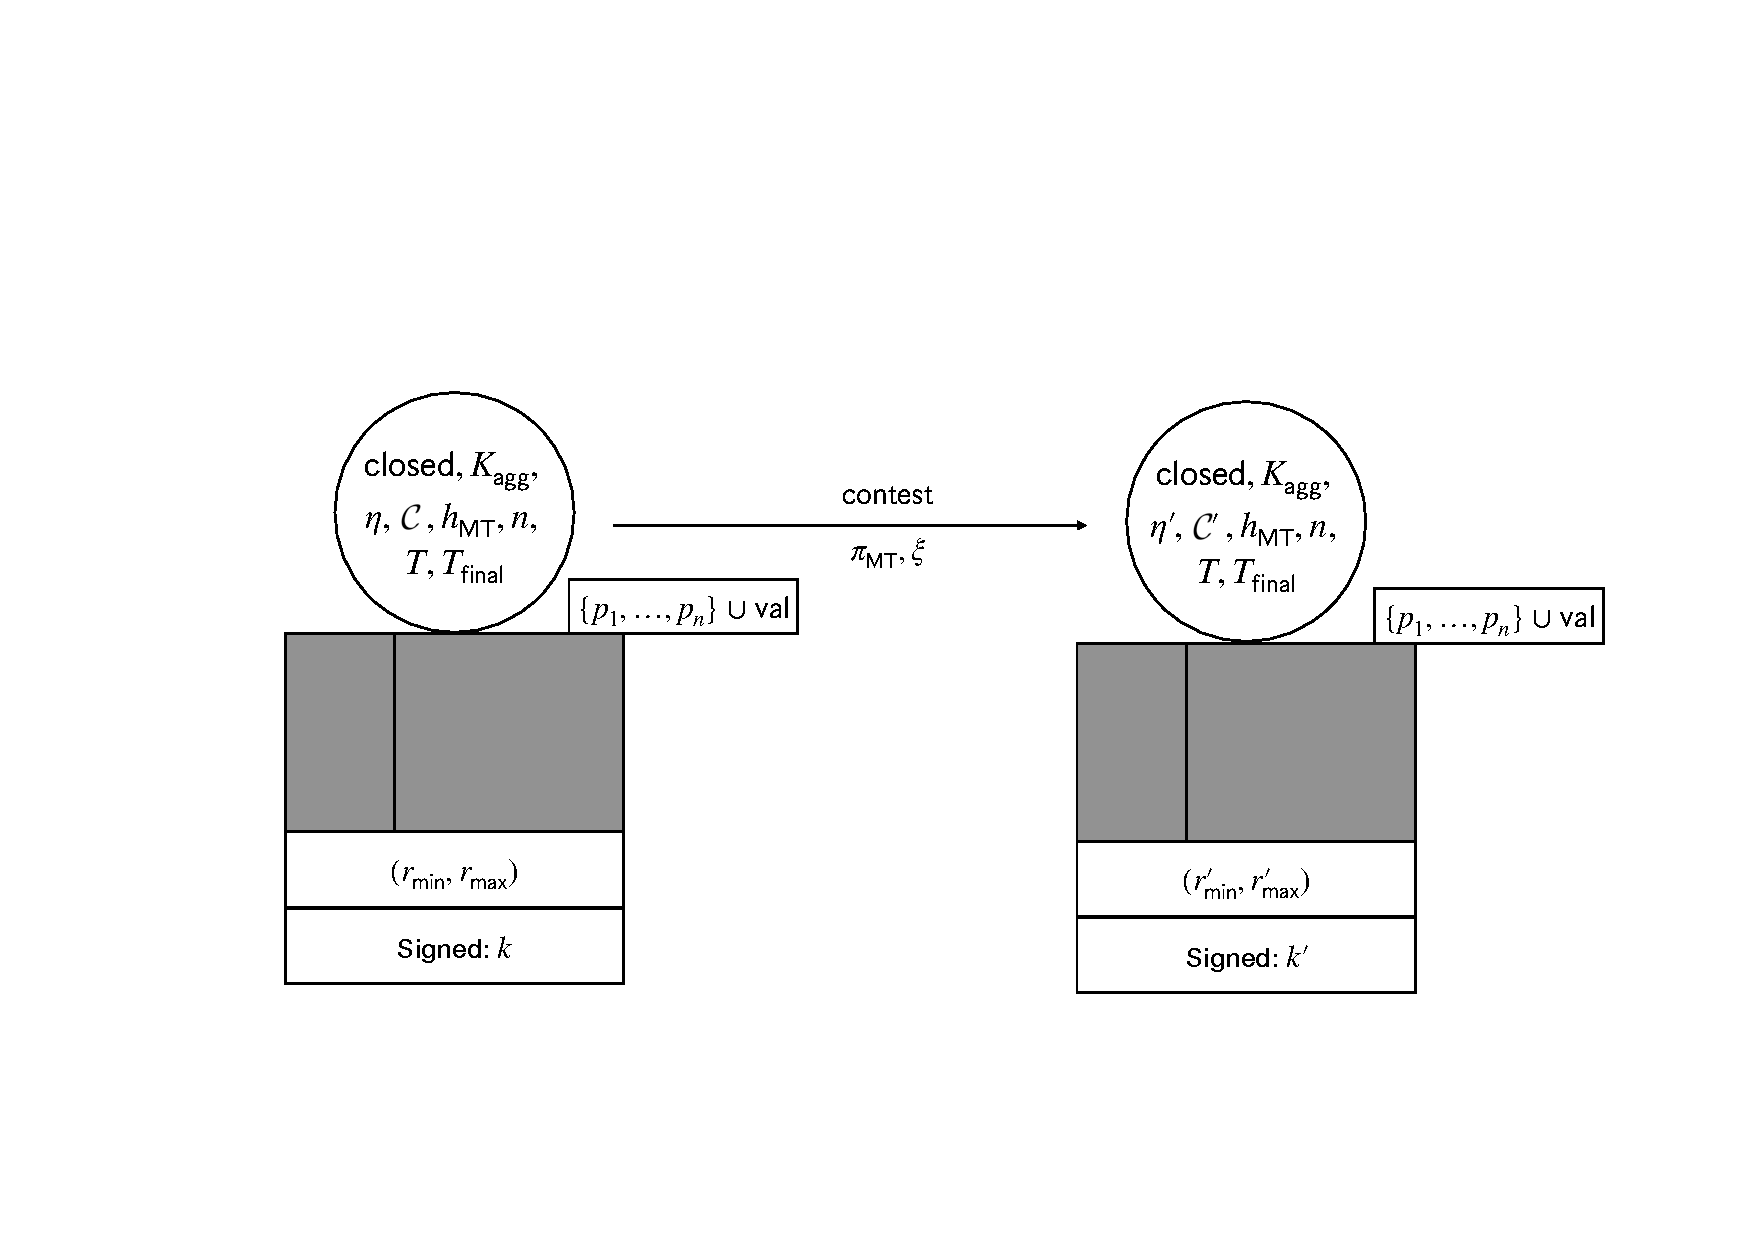
\includegraphics[width=\textwidth/2]{figures/SM_closed_closed.pdf}

  \caption{\mtxClose{}/\mtxContest{} transaction (left);
    \mtxContest{} transaction (right)}
  \label{fig:SM_closed_closed}

\end{figure}



%%% Local Variables:
%%% mode: latex
%%% TeX-master: "main"
%%% End:


The \mtxContest{} transaction (see Figure~\ref{fig:SM_closed_closed}) is posted
by a party to prove the currently $\stClosed$ state is not the latest one. This
transaction has a single input spending from the $\nuHead$ and paying to the
$\nuHead$ validator, which checks the state of the CEM is advanced:
\[
  (\stClosed,\cid,\hpAK,\hppuv,\nop,\cPer,\eta_0,\eta,\contesters,\Tfinal) \xrightarrow[\xi]{\mathsf{contest}} (\stClosed,\cid,\hpAK,\hppuv,\nop,\cPer,\eta_0,\eta',\contesters',\Tfinal')
\]

\noindent The $\nuHead$ validator performs these checks:
\begin{menumerate}
  \item Contest snapshot is newer $s' > s$, where $(s, \cdot) = \eta$ is the current and $(s', \cdot) = \eta'$ is the contest snapshot number
  \item $\xi$ is a valid multi-signature of the new snapshot state
  $\msVfy(\hpAK,(\cid || \eta_{0} || \eta'),\xi) = \true$
  \item The single signer $\{\keyHash\} = \txKeys$ has not already contested $\keyHash \not\in \contesters$ and is added to the set of contesters $\contesters' = \contesters \cup \keyHash$
  \item Transaction is posted before deadline $\txRmax \leq \Tfinal$
  \item Contestation deadline is updated correctly
     \[
       \Tfinal' = \left\{\begin{array}{ll}
                           \Tfinal     & \mathrm{if} ~ |\contesters'| = n, \\
                           \Tfinal + T & \mathrm{otherwise}
                         \end{array}\right.
    \]
  \item Transaction is signed by a participant $\exists (\cid \rightarrow \keyHash_{i} \rightarrow 1) \in \val' \Rightarrow \keyHash_{i} \in \txKeys$
  \item Value in the head is preserved $\val' = \val$
  \item No minting or burning $\txMint = \varnothing$
\end{menumerate}

\subsection{Fan-Out Transaction}

\begin{figure}

  \centering

  % 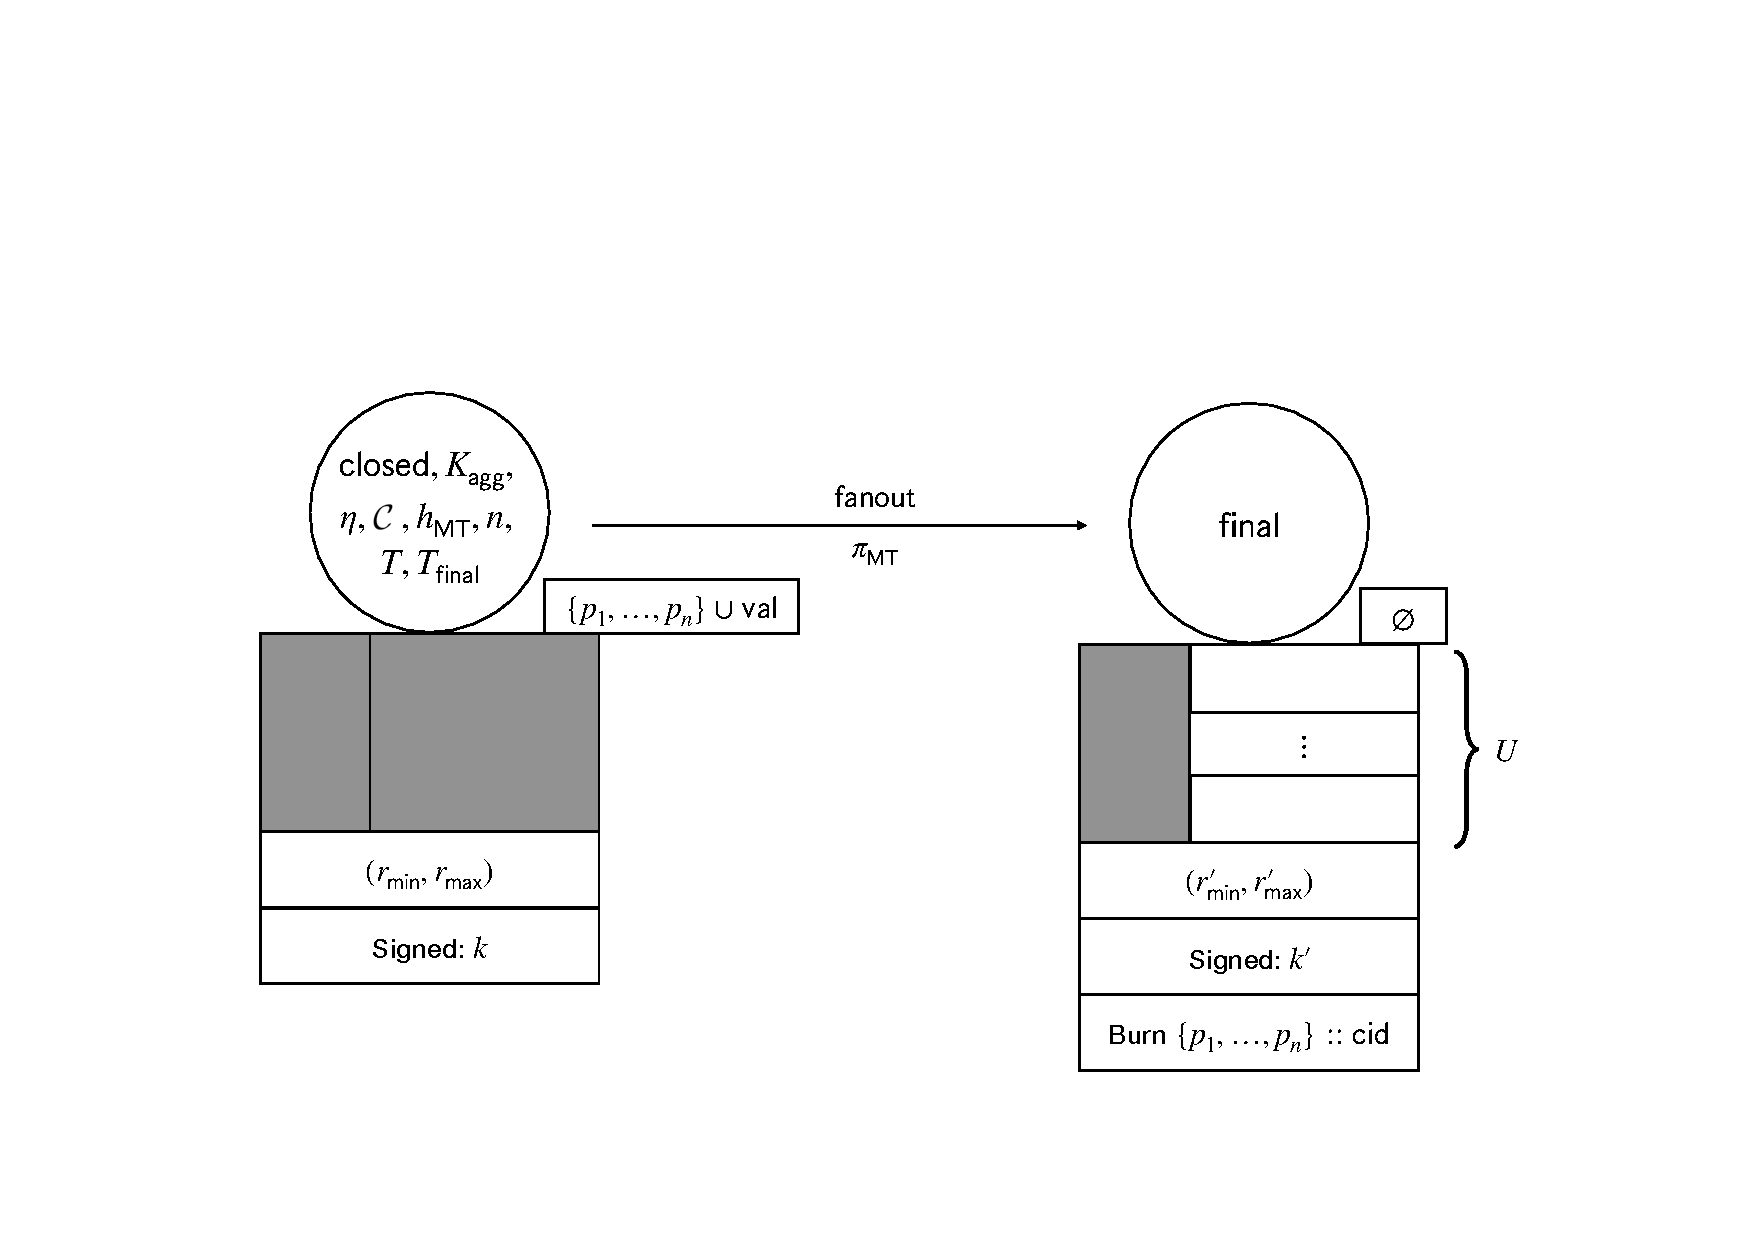
\includegraphics[width=\textwidth/2]{figures/SM_closed_final.pdf}

  % TODO: clean draw marked up version
  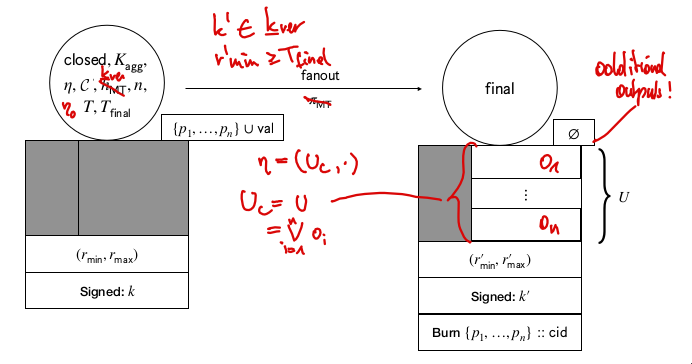
\includegraphics[width=\textwidth/2]{figures/SM_closed_final.png}

  \caption{\mtxClose{}/\mtxContest{} transaction (left);
    \mtxFanout{} transaction (right)}\label{fig:SM_closed_final}

\end{figure}

%%% Local Variables:
%%% mode: latex
%%% TeX-master: "main"
%%% End:


\noindent Once the contestation phase is over, a head may be finalized by posting a
\mtxFanout{} transaction (see Figure~\ref{fig:SM_closed_final}), which
distributes UTxOs from the head according to the latest state. It consists of
\begin{itemize}
  \item one input spending from $\nuHead$ holding the $\st$, and
  \item $m$ outputs to fan-out UTxOs.
\end{itemize}
Note that \mtxFanout{} represents a final transition of the CEM and hence there
is no state machine output. The input spending from $\nuHead$ does provide the
number of fanned-out outputs $m$ as redeemer and checks the state of the CEM is
advanced to the final $\stFinal$ as follows:
\[
  (\stClosed,\cid,\hpAK,\hppuv,\nop,\cPer,\eta_0,\eta,\contesters,\Tfinal) \xrightarrow[m]{\mathsf{fanout}} \stFinal,
\]

\noindent The $\nuHead$ validator performs these checks:
\begin{enumerate}
  \item The first $m$ outputs are distributing funds according to
        $(\cdot, U^{\#}) = \eta$\todo{explain ordering?}
        \[
        \hash(\bigoplus_{j=1}^{m} \bytes(\txOutputs[j])) = U^{\#}
        \]
  \item Transaction is posted after contestation deadline $\txRmin > \Tfinal$
  \item All tokens are burnt
        $|\{\cid \rightarrow \cdot \rightarrow -1\} \in \txMint| = n + 1$\todo{number
        of tokens burned vs. explicit enumeration what to burn?}
\end{enumerate}

%%% Local Variables:
%%% mode: latex
%%% TeX-master: "main"
%%% End:

\section{Off-Chain Protocol}\label{sec:offchain}

This section describes the actual Coordinated Hydra Head protocol, an even more
simplified version of the original publication~\cite{hydrahead20}. See the
protocol overview in Section~\ref{sec:overview} for an introduction and notable
changes to the original protocol. While the on-chain part already describes the
full life-cycle of a Hydra head on-chain, this section completes the picture by
defining how the protocol behaves off-chain and notably the relationship between
on- and off-chain semantics. The protocol is specified as a reactive system that
processes three kinds of events:
\begin{enumerate}
  \item on-chain protocol transactions as introduced in
        Section~\ref{sec:on-chain}, which are posted to the mainchain and can be
        observed by all actors
  \item off-chain network messages sent between protocol actors (parties):
    \begin{itemize}
      \item $\hpRT$: to request a transaction to be included in the next snapshot
      \item $\hpRS$: to request a snapshot to be created \& signed by every head member
      \item $\hpAS$: to acknowledge a snapshot by replying with their signatures
    \end{itemize}
  \item client commands as received from the environment
    \begin{itemize}
      \item $\hpInit$: to start initialization of a head
      \item $\hpNew$: to submit a new transaction to an open head
      \item $\hpClose$: to request closure of an open head
    \end{itemize}
\end{enumerate}
\todo{add a state diagram?}

The behavior is fully specified in Figure~\ref{fig:head_coordinated}, while the
following paragraphs introduce notation and explain variables.

\subsection{Assumptions}

On top of the statements of the protocol setup in Section~\ref{sec:setup}, the
off-chain protocol logic relies on these assumptions:
\todo{move some/merge with protocol setup?}
\begin{itemize}
  \item Every network message received from a specific party is checked for
        authentication. An implementation of the specification needs to find a
        suitable means of (channel) authentication. Unauthenticated messages are
        dropped.
  \item The head protocol gets correctly (and with completeness) notified about
        observed transactions on-chain belonging to the respective head
        instance.
  \item The specification covers only a single instance of a Hydra head.
        However, some implementations may choose to track multiple instances. As
        multiple Hydra heads might exist on the same blockchain, it is vital
        that they do not interfere and the specification will take special care
        to ensure this.
  \item All events are processed to completion, i.e.\ run-to-completion semantics
        without preemption.
  \item Events are deduplicated. That is, any two identical events must not lead
        to multiple invocations of the handling semantics.
  \item Given the specification, events may pile up forever and implementations
        need to consider these situations (i.e.\ potential for DoS). Note that,
        from a security standpoint, these situations are identical to a
        non-collaborative peer.
  \item The lifecycle of a Hydra head on-chain does not cross (hard fork)
        protocol update boundaries. Note that these events are announced in
        advance hence it should be possible for implementations to react in such
        a way as to expedite closing of the head before such a protocol update.
        This further assumes that the contestation period parameter is picked
        accordingly.
\end{itemize}

\subsection{Notation}
\todo{missing:, apply tx, projection, map access}
\begin{itemize}
  \item $\KwOn~event$ specifies how the protocol reacts on a given $event$.
        Further information may be available from the constituents of $event$
        and origin of the event.
  \item $\Req~p$ means that boolean expression $p \in \tyBool$ must be satisfied
        for the further execution of a routine, while discontinued on $\neg p$.
  \item $\KwWait~p$ is a \todo{blocking in GDoc?} non-blocking wait for boolean
        predicate $p \in \tyBool$ to be satisfied. On $\neg p$, the execution of
        the routine is stopped, queued, and reactivated at latest when $p$ is
        satisfied.
  \item $\Multi{}~msg$ means that a message $msg$ is (channel-) authenticated
        and sent to all participants of this head, including the sender.
  \item $\PostTx{}~tx$ has a party create transaction $tx$, potentially from
        some data, and submit it on-chain. See Section~\ref{sec:on-chain} for
        individual transaction details. \todo{fail not used anymore? do we need
        it?}
  \item $\Out{}~event$ signals an observation of $event$, which is used in the
        security definition and proofs of Section~\ref{sec:security}.
\end{itemize}

\subsection{Variables}

Besides parameters agreed in the protocol setup (see Section~\ref{sec:setup}), a
party's local state consists of the following variables:

\todo{missing: $\tilde{\sigma}$, $\barmU$, $\hatmU$}
\begin{itemize}
  \item $\hats$: Sequence number of seen snapshot.
  \item $\bars$: Sequence number of confirmed snapshot.
  \item $\hatmL$: Local ledger state used to validate new and requested
        transactions against.
  \item $\mT_{all} \in {(\tyBytes \times \mT)}^{*}$: Set of all transactions,
        indexed by their transaction id, ever received via $\mathtt{reqTx}$
        (independent of their validity).\todo{needed? prune by removing from
        $\hatmT$?}
  \item $\hatmT \in {(\tyBytes \times \mT)}^{*}$: Set of transactions, indexed by
        their transaction id, that extend from the last confirmed snapshot
        $\barmU$ to form $\hatmL$. These are also the transactions that would go
        into the next snapshot (if this party is the next leader).
  \item $\Sigma \in {(\tyNatural \times \tyBytes)}^{*}$: Accumulator of signatures, indexed by parties.
\end{itemize}

\subsection{Protocol flow}

\todo{write about rollbacks}

\subsubsection{Initializing the head}

\dparagraph{$\hpInit$.}\quad Before a head can be initialized, all
parties need to exchange and agree on protocol parameters during the protocol
setup phase (see Section~\ref{sec:setup}), so we can assume the public Cardano
keys $\cardanoKeys^{setup}$, Hydra keys $\hydraKeysAgg^{setup}$, as well as the contestation
period $\cPer^{setup}$ are available. One of the clients then can start head initialization using the $\hpInit$ command, which will result in an $\mtxInit$ transaction being posted.\\

\dparagraph{$\mathtt{initialTx}$.}\quad All parties will receive this $\mtxInit$
transaction and validate announced parameters against the pre-agreed $setup$
parameters, as well as the structure of the transaction and the minting policy
used. This is a vital step to ensure the initialized Head is valid, which
cannot be checked completely on-chain (see also Section~\ref{sec:init-tx}). \\

\dparagraph{$\mathtt{commitTx}$.}\quad As each party $p_{j}$ posts a
$\mtxCommit$ transaction, the protocol records observed committed UTxOs of each
party $U_j$. With all committed UTxOs known, the $\eta$-state is created (as
defined in Section~\ref{sec:collect-tx}) and the $\mtxCollect$ transaction is
posted. Note that while each participant may post this transaction, only one of
them will be included in the blockchain as the mainchain ledger prevents double
spending. Should any party want to abort, they would post an $\mtxAbort$
transaction and the protocol would end at this point.\\

\dparagraph{$\mathtt{collectComTx}$.}\quad Upon observing the $\mtxCollect$
transaction, the parties compute $\Uinit \gets \bigcup_{j=1}^{n} U_j$ using
previously observed $U_j$ and initialize $\hatmU = \barmU = \hatmL = \Uinit$
with it\todo{check $\eta$ against $\Uinit$?}. The initial transaction sets are
empty $\mT = \barmT =\hatmT =\emptyset$, and $\bars = \hats = 0$.

\subsubsection{Processing transactions off-chain}

Transactions are announced and captured in so-called snapshots. Parties generate
snapshots in a strictly sequential round-robin manner. The party responsible for
issuing the $\ith i$ snapshot is the \emph{leader} of the $\ith i$ snapshot.
While the frequency of snapshots in the general Head protocol~\cite{hydrahead20}
was configurable, the Coordinated Head protocol does specify a snapshot to be
created after each transaction.\\

\dparagraph{$\hpNew$.}\quad At any time, by sending request $(\hpNew,\tx)$, a
head party can (asynchronously) submit a new transaction $\tx$ to the head
protocol. For this, the transaction must be well-formed ($\validTx$)\todo{remove
  $\validTx$?} and applicable to the current local ledger state
$\hatmL \applytx \tx \neq \bot$. If the checks
pass, a $(\hpRT,\tx)$ message is sent out to all parties.\\

\dparagraph{$\hpRT$.}\quad Upon receiving request $(\hpRT,\tx)$, the transaction gets
recorded in $\mT$ and $\barmT$ using the tx hash $tx^{\#} = \hash(tx)$ and applied to the
local \emph{seen} ledger state $\hatmL \applytx \tx$. If there is no current
snapshot ``in flight'' ($\hats = \bars$) and the receiving party $i$ is the next
snapshot leader, a message to request snapshot signatures $\hpRS$ is sent. Note
that only transaction hashes are submitted in this message. \\

\dparagraph{$\hpRS$.}\quad Upon receiving request $(\hpRS,s,\mT^{\#}_{req})$
from party $\party_j$, the receiver $\party_i$ checks that $s$ is the next
snapshot number and that party $\party_j$ is responsible for leading its
creation.\todo{define $\hpLdr$?} Party $\party_i$ then waits until the previous
snapshot is confirmed ($\bars = \hats$) and all transactions referred by hashes
in $\mT^{\#}_{req}$ are resolvable to $\mT_{res}$\todo{also "output seen" for
  security}. Only then, $\party_i$ increments their seen-snapshot counter
$\hats$, resets the signature accumulator $\Sigma$, and computes the UTxO set
$\hatmU$ of the new (seen) snapshot as $\hatmU \gets \barmU \applytx \mT_{res}$.
Then, $\party_i$ creates a signature $\msSig_i$ using their signing key
$\hydraSigningKey$ on a message comprised by the $\cid$, the $\eta_{0}$
corresponding to the initial UTxO set $\Uinit$, and the new $\eta'$ given by the
new snapshot's number $\hats$ a canonically combining $\hatmU$ (see
Section~\ref{sec:close-tx} for details). The signature is sent to \emph{all}
head members via message $(\hpAS,\hats,\msSig_i)$. Note that no UTxO sets have
to be exchanged in this process as the parties all locally compute a new
snapshot by the given transaction hashes. Finally, the pending transaction set
$\hatmT$ gets pruned by the just requested transactions $\mT_{res}$ and the
local ledger state $\hatmL$ is updated accordingly.\\

\dparagraph{$\hpAS$.}\quad Upon receiving acknowledgment $(\hpAS,s,\msSig_j)$,
all participants $\Req$ that it is from an expected snapshot (either the last
seen $\hats$ or + 1), the signature is not yet included in $\Sigma$, and
potentially $\KwWait$ for the corresponding $\hpRS$ such that $\hats = s$. They
store the received signature in the signature accumulator $\Sigma$. If a
signature from each party has been collected, $\party_i$ aggregates the
multisignature $\msCSig$ and $\Req$ it to be valid. \todo{detect cheating (fail)
  here?} If everything is fine, the snapshot can be considered confirmed
\todo{output conf for all txs for security definition} by updating $\bars=s$ and
storing everything for later reference in $\barmU$ \todo{different variable
  name?}. Similar to the $\hpRT$, if $\party_i$ is the next snapshot leader and
there are already transactions to snapshot in $\hatmT$, a corresponding $\hpRS$
is distributed.

\subsubsection{Closing the head}

\dparagraph{$\hpClose$.}\quad In order to close a head, a client issues the
$\hpClose$ event which uses the latest confirmed snapshot $\barmU$ to create
\begin{itemize}
  \item the new $\eta$-state $\eta'$ from the last confirmed UTxO set and snapshot
        number, and
  \item the certifiate $\xi$ using the corresponding multi-signature.
\end{itemize}
With $\eta'$ and $\xi$, the $\mtxClose$ transaction can be constructed and
posted. See Section~\ref{sec:close-tx} for details about this transaction. \\

\dparagraph{$\mathtt{closeTx}/\mathtt{contestTx}$.}\quad When a party observes
the head getting closed or contested, the $\eta$-state extracted from the
\mtxClose{} or \mtxContest{} transaction represents the latest head status that
has been aggregated on-chain so far (by a sequence of \mtxClose{} and
\mtxContest{} transactions). If the last confirmed (off-chain) snapshot is newer
than the observed (on-chain) snapshot number $s_{c}$, an updated $\eta$-state
and certificate $\xi$ is constructed posted in a \mtxContest{} transaction (see
Section~\ref{sec:contest-tx}).

\begin{figure*}[t!]

  \def\sfact{0.8}
  \centering
  \begin{algobox}{Coordinated Hydra Head}
    \medskip
    \begin{tabular}{c}
      %%% Initializing the head
      \begin{tabular}{cc}
        \adjustbox{valign=t,scale=\sfact}{
         \begin{walgo}{0.6}
          %%% INIT
           \On{$(\hpInit,\hydraKeys,\hydraSigningKey,\cardanoKeys,\cPer)$ from client}{ %
             $\hydraKeysAgg^{setup} \gets \msCombVK(\hydraKeys)$ \; %
             $\cardanoKeys^{setup} \gets \cardanoKeys$ \; %
             $\cPer^{setup} \gets \cPer$ \; %
            $\PostTx{}~(\mtxInit, \nop, \hydraKeysAgg,\cardanoKeys,\cPer)$ \; %
          }
          \vspace{12pt}

          \On{$(\gcChainInitial, \cid, \nop, \hydraKeysAgg, \cardanoKeys^{\#}, \cPer)$ from chain}{ %
           \Req{} $\hydraKeysAgg=\hydraKeysAgg^{setup}$\; %
           \Req{} $\cardanoKeys^{\#}= [ \hash(k)~|~\forall k \in \cardanoKeys^{setup}]$\; %
           \Req{} $\cPer=\cPer^{setup}$\; %
           % TODO: cid check good enough?
           \Req{} $\cid = \hash(\muHead(i_{seed}))$ \; %
          }
        \end{walgo}
        }
        &

        \adjustbox{valign=t,scale=\sfact}{
        \begin{walgo}{0.6}
          \On{$(\gcChainCommit, j, U)$ from chain}{ %
            $U_j \gets U $

            \If{$\forall k \in [1..n]: U_k \neq \undefined$}{ %
              $\eta \gets (0, \combine([U_1 \dots U_n]))$ \; %
              $\PostTx{}~(\mtxCCom, \eta)$ \; %
            } %
          }

          \vspace{12pt}

          \On{$(\gcChainCollectCom, \eta_{0})$ from chain}{ %
            \Req{} $\forall j \in [1..n]: U_j \neq \undefined$ \; %
            $\Uinit \gets \bigcup_{j=1}^{n} U_j$ \; %
            $\hatmU, \barmU, \hatmL \gets \Uinit$ \; %
            $\hats,\bars \gets 0$ \; %
            $\mT, \hatmT, \barmT \gets \emptyset$ \;
          }

        \end{walgo}
      }
      \end{tabular}
      
      \\
      \multicolumn{1}{l}{\line(1,0){490}} %
      \\

      %%% Open head
      \begin{tabular}{c@{}c}
        \adjustbox{valign=t,scale=\sfact}{
        \begin{walgo}{0.65}

          %%% NEW TX
          \On{$(\hpNew,\tx)$ from client}{%
            \Req{} $\validTx(\tx) \land \hatmL \applytx \tx \neq \bot$\;
            \Multi{} $(\hpRT,\tx)$%
          }

          \vspace{12pt}

          %%% REQ TX
          \On{$(\hpRT,\tx)$ from $\party_j$}{%
            \Req{} $\validTx(\tx) \land \hatmL \applytx \tx \neq \bot$ \;

            $\tx^{\#} \gets \hash(\tx)$ %

            $\mT \gets \mT \cup (\tx^{\#}, \tx)$ % all seen txs

            $\hatmT \gets \hatmT \cup (\tx^{\#}, \tx)$ % candidates for next snapshot

            $\hatmL \gets \hatmL\applytx\tx$ %

            % issue snapshot if we are leader
            \If{$\hats = \bars \land \hpLdr(\bars + 1) = i$}{%
              \Multi{} $(\hpRS,\bars+1,\hatmT^{\downarrow1})$ \;%
            }
          }

          \vspace{12pt} %

          %%% REQ SN
          %TODO: avoid hash resolution complexity? it's handwavy at best right now
          \On{$(\hpRS,s,\mT^{\#}_{req})$ from $\party_j$}{ %

            \Req{} $s = \hats + 1 \land \hpLdr(s) = j$ \; %


            % Wait for snapshot no snapshot in flight anymore and all txs resolvable
            \Wait{$\bars = \hats \land \forall h \in \mT^{\#}_{req} : (h, \cdot) \in \mT$}{ %

              % resolve requested transactions
              $\mT_{res} \gets [ \mT[h] ~ | ~ \forall h \in \mT^{\#}_{req}]$

              \Wait{$\barmU \applytx \mT_{res} \not= \bot$}{ %
                $\hats \gets \bars + 1$ \; %

                $\hatmU \gets \barmU \applytx \mT_{res}$ \; %

                $\eta' \gets (\hats, \combine(\hatmU))$ \; %
                $\msSig_i \gets \msSign(\hydraSigningKey, (\cid || \eta_{0} || \eta'))$ \; %
                $\hatSigma \gets \emptyset$

                $\Multi{}~(\hpAS,\hats,\msSig_i)$ \; %

                $\forall \tx \in \mT_{res}: \Out~(\hpSeen,\tx)$ \; %

                % TODO: pruning is handwavy
                $\hatmT :\subseteq_{\mbox{max}} \mT$ s.t. $\hatmU\applytx\hatmT\not=\bot$ \; %
                $\hatmL \gets \hatmU\applytx\hatmT$
              }
            }
           }
          
        \end{walgo}
        }
        &

        \adjustbox{valign=t,scale=\sfact}{
        \begin{walgo}{0.6}
          %%% ACK SN
          \On{$(\hpAS,s,\msSig_j)$ from $\party_j$}{ %

            \Req{} $s \in \{\hats,\hats+1\} ~ \land ~ (j,\msSig_j) \notin \hatSigma$
            \; %

            \Wait{$\hats=s$
            }{ %
            

            $\hatSigma \gets \hatSigma \cup (j,\msSig_j)$ \; %

            \If{$\forall k \in [1..n]: (k,\cdot) \in \hatSigma$}{ %
              $\msCSig \gets \msComb(\hydraKeys, \hatSigma)$ \; %

              $\eta' \gets (\hats, \combine(\hatmU))$ \; %
              \Req{} $\msVfy(\msCVK, (\cid || \eta_{0} || \eta'), \msCSig)$ \;
              $\barmU \gets \hatmU$ \; %
              $\bars \gets \hats$ \; %
              $\barsigma \gets \msCSig$ \; %

              $\forall \tx \in \mT_{res} : \Out (\hpConf,\tx)$ \; %

              % issue snapshot if we are leader
              \If{$\hats = \bars \land \hpLdr(\bars + 1) = i$}{%
                \Multi{} $(\hpRS,\bars+1,\hatmT^{\downarrow1})$ \;%
              }
            }
          } }
        \end{walgo}

          }

      \end{tabular}

      \\
      \multicolumn{1}{l}{\line(1,0){490}} %
      \\

      %%% Closing the head
      \begin{tabular}{c c}
        \adjustbox{valign=t,scale=\sfact}{
        \begin{walgo}{0.6}

          % CLOSE from client
          \On{$(\hpClose)$ from client}{ %
            $\eta' \gets (\bars, \combine(\barmU))$ \; %
            $\xi \gets \barsigma$ \; %
            $\PostTx{}~(\mtxClose, \eta', \xi)$ \; %
          }

        \end{walgo}
        }
        & \adjustbox{valign=t,scale=\sfact}{
          \begin{walgo}{0.6}

          \On{$(\gcChainClose, \eta) \lor (\gcChainContest, \eta)$ from chain}{ %
            $(s_{c}, \cdot) \gets \eta$ \;
            \If{$\bars > s_{c}$}{%
              $\eta' \gets (\bars, \combine(\barmU))$ \; %
              $\xi \gets \barsigma$ \; %
              $\PostTx{}~(\mtxContest, \eta', \xi)$ \; %
            } }

          \end{walgo}
          }
      \end{tabular}
    \end{tabular}
    \bigskip
  \end{algobox}
  
  \caption{Head-protocol machine for the \emph{coordinated head} from the
    perspective of party $\party_i$.}\label{fig:head_coordinated}

\end{figure*}



%%% Local Variables:
%%% mode: latex
%%% TeX-master: "main"
%%% End:


%%% Local Variables:
%%% mode: latex
%%% TeX-master: "main"
%%% End:

% TODO: disabled \section{Security (WIP --- Iteration 1)}\label{sec:security}

\todo{Add security experiment}
\noindent Adversaries:

\begin{mdescription}
\item[Active Adversary.] An \emph{active adversary} $\adv$ has full control
  over the protocol, i.e., he is fully unrestricted in the above security game.

 \item[Network Adversary.] A \emph{network adversary} $\adv_\emptyset$ does not corrupt
   any head parties, eventually delivers all sent network messages
   (i.e., does not drop any messages), and does not cause the $\hpClose$ event.
   Apart from this restriction, the adversary can act arbitrarily in the above experiment.
\end{mdescription}

\noindent Random variables:

\begin{mitemize}
\item $\That_i$: the set of transactions $\tx$ for which party $\party_i$,
  \emph{while uncorrupted}, output $(\hpSeen,\tx)$;

\item $\Tbar_i$: the set of transactions $\tx$ for which party $\party_i$,
  \emph{while uncorrupted}, output $(\hpConf,\tx)$;
    
\item $\Snapbar_i$: latest snapshot $(s,U)$ that party
  $\party_i$ performed \emph{while uncorrupted}: output $(\hpSnap,(s,U))$;

\item $\Hcont$: the set of (at the time) uncorrupted parties who produced
  $\xi$ upon close/contest request and $\xi$ was applied to
  correct~$\eta$; and

\item $\honest$: the set of parties that remain uncorrupted.
\end{mitemize}


\noindent Security conditions / events:

\begin{itemize}
\item \propName{Consistency (Head)}: In presence of an active adversary, the
  following condition holds at any point in time:
   For all $i,j$,
   $\Uinit \circ (\Tbar_i \cup \Tbar_j) \not= \bot$, i.e., no two
   uncorrupted parties see conflicting transactions confirmed.

  \item \propName{Oblivious Liveness (Head)}:
    Consider any protocol execution in presence of a network adversary wherein
    the head does not get closed for a sufficiently long period of time, and consider
    an honest party $p_i$ who enters transaction $\tx$ by executing $(\hpNew,\tx)$ \emph{each time after having finished a snapshot}.

    Then the following eventually holds:
    $\tx \in \bigcap_{i\in[n]} \Tbar_i\ \vee\ %
    \forall i: \Uinit \circ (\Tbar_i\cup\{\tx\}) = \bot$,
    i.e., every party will observe the transaction confirmed or every party
    will observe the transaction in conflict with their confirmed transactions.\footnote{
      In particular, \emph{liveness} expresses that the protocol makes progress
      under reasonable network conditions if no head parties get corrupted.
    }

\item \propName{Soundness (Chain)}: In presence of an active adversary,
  the following condition is satisfied:
  $\exists \Ttilde \subseteq \bigcap_{i \in \honest} \That_i : \Ufinal
  = \Uinit \circ \Ttilde\not=\bot$, i.e., the final UTxO set results
  from applying a set of transactions to $U_0$ that have been seen by
  all honest parties (wheras each such transaction applies conforming to the ledger rules).
\item \propName{Completeness (Chain)}: In presence of an active adversary,
  the following condition holds: For $\Ttilde$ as above,
  $\bigcup_{p_i \in \Hcont} \Tbar_i \subseteq \Ttilde$, i.e., all
  transactions seen as confirmed by an honest party at the end of the
  protocol are considered.
\end{itemize}

Note that the original version of the coordinated head satisfies a stronger version of liveness which is important for the 'user experience' in the protocol:
\begin{itemize}
  \item \propName{Liveness (Head)}:
    Consider any protocol execution in presence of a network adversary wherein
    the head does not get closed for a sufficiently long period of time, and consider
    an honest party $p_i$ who enters transaction $\tx$ by executing $(\hpNew,\tx)$.

    Then the following eventually holds:
    $\tx \in \bigcap_{i\in[n]} \Tbar_i\ \vee\ %
    \forall i: \Uinit \circ (\Tbar_i\cup\{\tx\}) = \bot$,
    i.e., every party will observe the transaction confirmed or every party
    will observe the transaction in conflict with their confirmed transactions.\footnote{
      In particular, \emph{liveness} expresses that the protocol makes progress
      under reasonable network conditions if no head parties get corrupted.
    }
\end{itemize}


\subsection{Proofs}

\paragraph{Consistency.}

\begin{lemma}[Consistency]
  \label{lem:consistency}
  The coordinated head protocol satisfies the \propName{Consistency} property.
\end{lemma}
\begin{proof}
  Observe that $\Tbar_i\cup\Tbar_j\subseteq\That_i$ since no
  transaction can be confirmed without every honest party signing off
  on it.  Since parties do not sign conflicting transactions
  (see $\hpRS$, `wait'), we have
  $\Uinit\applytx\Tbar_i\neq\bot$,
  $\Uinit\applytx\Tbar_j\neq\bot$, and
  $\Uinit\applytx\That_i\neq\bot$.  Thus, since $\Tbar_i\cup\Tbar_j\subseteq\That_i$
  it follows that
  $\Uinit\applytx(\Tbar_i\cup\Tbar_j)\neq\bot$
\end{proof}

\paragraph{Oblivious Liveness.}
For all lemmas towards oblivious liveness, we assume the presence of a network adversary, and that the head does not get closed for a sufficiently
long period of time.
We call this the \emph{liveness condition}.

\begin{lemma}\label{lem:reqconf}  
  Under the liveness condition, any snapshot issued as $(\hpRS,s,T)$ will eventually be confirmed
  in the sense that every party holds a valid mulisignature on it.
\end{lemma}
\begin{proof}
  Consider a party $p_i$ receiving message $(\hpRS,s,T)$. We demonstrate that $p_i$ executes
  the code past the `wait' instruction of the $\hpRS$ routine. 

  \begin{itemize}
   \item Passing the `require' guard:
  Note that the snapshot leader sends the request only if $\hats=\bars$, and for $s=\hats+1$.
  Thus, $\hats_i=\hats$ since $p_i$ has already signed the snapshot for $\hats$. The `require'
  guard is thus satisfied for $p_i$.

   \item Passing the `wait' guard:
  Since the snapshot leader sees $\hats=\bars$, also $p_i$ will eventually see $\hats_i=\bars_i$. Furthermore, since all leaders are honest, it holds that $\hatmU\applytx\mT_{res}\not=\bot$ by construction.
  \end{itemize}

  This implies that every party will eventually sign and acknowledge the newly created snapshot.
  Finally, the `require' and `wait' guards of the $\hpAS$ code will be passed by every party
  since an $\hpAS$ for snapshot number $s$ can only be received for $s\in\{\hats,\hats+1\}$
  as an acknowledgement can only be received for the current snapshot being worked on by $p_i$
  or a snapshot that is one step ahead---implying that everybody will hold a valid multisignature
  on the snapshot in consideration.
\end{proof}

\begin{lemma}[Eternal snapshot confirmation]\label{lem:eternal}
  Under the liveness condition, as long as new transactions are issued, for any $k>0$, every party eventually confirms
  a snapshot with sequence number $s=k$.
\end{lemma}
\begin{proof}
  By Lemma~\ref{lem:reqconf}, any requested snapshot eventually gets confirmed, implying
  that the next leader observes $\hats=\bars$ and thus, in turn, issues a new snapshot.
  Thus, for any $k$, a snapshot is eventually confirmed.
\end{proof}

\begin{lemma}[Oblivious Liveness]
  \label{lem:liveness}
  The coordinated head protocol satisfies the \propName{Oblivious Liveness} property.
\end{lemma}
\begin{proof}
  Consider the first point in time where a transaction $\tx$ enters the system by some party $p_i$
  issuing $(\hpNew,\tx)$, and consider the next point in time
  $t$ when $p_i$ issues a snapshot.

  By Lemma~\ref{lem:eternal}, this snapshot will eventually be issued and confirmed by all parties.
  
  \medskip
  
  Let $\hatmT$ be the transactions to be considered by $p_i$'s snapshot: $\hatmL=\barmU\applytx\hatmT$
  where $\barmU$ is the snapshot prior to $p_i$'s. Since $p_i$ issues
  $(\hpRT,\tx)$ after each snapshot, we have that, either,
  \begin{itemize}
      \item $\tx\in\hatmT$, in which case $\tx \in \bigcap_{i\in[n]} \Tbar_i$ after everybody has completed this snapshot, or,
      \item $\tx\notin\hatmT$, in which case $\hatmL\applytx\tx=\bot$ ($\tx$ is still in the wait queue of $(\hpRT,\tx)$. After everybody has completed this snapshot, it thus holds that $\forall i: \Uinit\applytx\bigcap_{i\in[n]}{\Tbar_i}=\hatmL$, and .
  \end{itemize}
  In both cases, the lemma follows.
\end{proof}

\paragraph{Soundness and completeness.}

\begin{lemma}[Soundness]
  \label{lem:soundness}
  The basic head protocol satisfies the \propName{Soundness} property.
\end{lemma}

\begin{proof}
  Let $T$ be the set of transactions such that $\Ufinal=U_0\applytx T$.
  Since $\Ufinal$ is multi-signed, it holds that $T\subseteq\That_i$
  ($T$ is \emph{seen}) by every honest party in the head.
  Furtermore, since honest signatures are only issued for valid transaction,
  $\Ufinal\not=\bot$ (i.e., $\Ufinal$ is a valid state), and soundness
  follows.
\end{proof}


\begin{lemma}[Completeness]
 \label{lem:completeness}
 The basic head protocol satisfies the \propName{Completeness}
 property.
\end{lemma}
\begin{proof}
  Consider all parties $p_i\in\Hcont$. Since the close/contest process
  finally accepts the latest multi-signed snapshot, it holds that
  $\Ufinal.s \geq \max_{p_i\in\Hcont}(\bars_i)$, and thus that
  $\bigcup_{p_i\in\Hcont}\Tbar_i\subseteq\bigcap_{p_i\in\honest}\That_i$,
  and completeness follows.
\end{proof}

%%% Local Variables:
%%% mode: latex
%%% TeX-master: "main"
%%% End:


\bibliographystyle{plain}
\bibliography{short}

\end{document}
